% ****** Start of file apssamp.tex ******
%
%   This file is part of the APS files in the REVTeX 4.1 distribution.
%   Version 4.1r of REVTeX, August 2010
%
\documentclass[reprint,%article
 %,
%superscriptaddress,
%groupedaddress,
%unsortedaddress,
%runinaddress,
%frontmatterverbose, 
%preprint,
%showpacs,preprintnumbers,
%nofootinbib,
%nobibnotes,
%bibnotes,
 amsmath,amssymb,
 aps,
%pra,
%prb,
%rmp,
%prstab,
%prstper,
%floatfix,
]{revtex4-1}
\usepackage[table,xcdraw]{xcolor}

%\usepackage{xcolor}

\usepackage{graphicx}% Include figure files
\usepackage{dcolumn}% Align table columns on decimal point
\usepackage{bm}% bold math
\usepackage{appendix}
\usepackage{subcaption}
%\usepackage{subfloat}
%\usepackage{hyperref}% add hypertext capabilities
%\usepackage[mathlines]{lineno}% Enable numbering of text and display math
%\linenumbers\relax % Commence numbering lines

%\usepackage[showframe,%Uncomment any one of the following lines to test 
%%scale=0.7, marginratio={1:1, 2:3}, ignoreall,% default settings
%%text={7in,10in},centering,
%%margin=1.5in,
%%total={6.5in,8.75in}, top=1.2in, left=0.9in, includefoot,
%%height=10in,a5paper,hmargin={3cm,0.8in},
%]{geometry}https://www.overleaf.com/project/5ba0361831a91c7b3990c0d7
 \usepackage{natbib}
 
\begin{document}

\preprint{APS/123-QED}

\title{DRAFT- Rotation Curve Fitting Model }% Force line breaks with \\
%\thanks{ Thanks Jesus}%

% Find out if Joe and Noah still want to be on this paper%

 

\author{Sophia Natalia Cisneros}
 \affiliation{ Department of Astronomy,  
 University of Washington}
 % \email{sophia.cisneros@du.edu}
  \author{Richard Ott}%
 \email{rich.ott@EMAIL.com}
\affiliation{Affiliate MIT - Ask Joe Formaggio}%Tech dudes \textbackslash\textbackslash
%}
 \author{ Meagan Crowley}
\email{ }
\affiliation{NREL}%
 \author{ Amy Roberts}
\email{ }
\affiliation{CU Denver}%
\author{Marcus Paz}
\author{Zaneeyiah Brown}
\author{Landon Joyal}
\author{Roberto Real Rico}
\author{Elizabeth Gutierrez-Gutierrez}
\author{ Phong Pham}
\author{Zac Holland}
\author{Amanda Livingston}
\author{Lily Castrellon}
\author{Shanon Rubin}
\author{Aaron Ashley}
\author{Dillon Battaglia}
%\affiliation{UMass Boston% with \\
%&}%
%
 
 
\date{\today}% It is always \today, today,
             %  but any date may be explicitly specified
             %%%%%%
%%%%%%%
%%%%%%
%%%%%%%
%%%%%%
%%%%%%%
\begin{abstract}
 
 
{\color{teal}   Github repo: Cisneros-Galaxy/RCFM     }

\begin{description}
\item[Usage]
Secondary publications and information retrieval purposes.
\item[PACS numbers]
May be entered using the \verb+\pacs{#1}+ command.
%\item[Structure]
%You may use the \texttt{description} environment to structure your abstract;
%use the optional argument of the \verb+\item+ command to give the category of each item. 
\end{description}
\end{abstract}

\pacs{Valid PACS appear here}% PACS, the Physics and Astronomy
                             % Classification Scheme.
%\keywords{Suggested keywords}%Use showkeys class option if keyword
                              %display desired
\maketitle

%\tableofcontents
%%%%%%NOTES TO DO
%%%make labels for figure axes. remove orange line through the data
%%%%%%
%%%%%%%%
%%%%%%
%%%%%%%
%%%%%%
%%%%%%
\section{Introduction  \label{sec:uno}}


%DARK MATTER

 The flat-rotation curve problem of spiral galaxies  is viewed as primary evidence for dark matter\cite{Rub,Bosma,1985ApJAlbada}. 
 The dark matter paradigm interprets the divergence of two velocity parameters inferred from  different    observations of light, spectra and photometry (see Fig.~\ref{fig:NGC2403}),     as characterizing a missing or ``dark'' mass component in rotationally supported galaxies. 
 Photometry leads to dynamics by model based mass-to-light ratios and the Poisson equation, which predict Keplerian orbital velocities    falling off outside of the stars. 
 Doppler shifted spectra yield rotation curve velocities  by the Lorentz Doppler shift formula, which gives velocities which do not fall-off outside of the stars. 
 The mismatch is accounted for with dark matter halos which dwarf the visible light many times over. 
 Dark matter particles are hypothesized to make up these halos, and to have a very low interaction probability with baryonic matter,  and so,  experiments are ever increasing   sensitivity to detect them \cite{Cebrian:2022brv}.  In the absence of a direct detection of a dark matter particle the paradoxes of dark matter models remain interesting. 
 
   
   The first paradox is best stated by 
  S. McGaugh  when they ask   ``Why is the luminous tail wagging the dark matter dog,  if dark matter dominates dynamics ?'' \cite{1999McGaugh,McGaugh2016RAR}. This is known as the  disk-halo conspiracy, and references the strange fact that knowledge  of 
 the luminous stellar   disk  completely determine the spherical dark matter halo \cite{2004ApJ...609..652M}.  
 A second, related paradox  is known as  the Universal Rotation Curve (URC)  \cite{salucci,Persic,1978Rubin,10.1111/j.1365-2966.2007.11696.x}, in which  a spectrum of 1,100 galaxy rotation curves
 inflect  about  the Milky Way's  anticipated rotation curve (Fig.~\ref{fig:URC}).  This phenomenological trend requires   fine tuning in dark matter models, where the gravity theory is   classical and yet
  small, less dense,  dwarf galaxies are proportionally more successful at dark matter halo accretion than     larger, bright,  centrally dense    galaxies. 
   This fine-tuning reduces dark matter model's   
   predictivity   \cite{MCGAUGH2021220}. 
 Classically in gravity,  mass accretion rates are proportional to total mass \cite{10.1093/mnras/stt2403}. 

  
 
     The leading   alternative    to dark matter theory  in the flat-rotation curve problem is   Modified Newtonian Dynamics (MOND) \cite{Milgrom}.  
     MOND    proposes    the   luminous mass is the only mass, but that there exists a 
     a changing  physical law of gravity,    on the vast distance scales of galaxies \cite{McGaugh_2014}. 
MOND uses only   a single, roughly constant free-parameter to represent the new acceleration scale for all spiral   galaxies  \cite{McGaugh2016RAR,2022A&A...664A..40M}. 
    This approach  is   predictive across a  broad  sample of galaxy rotation curves,  representing diverse    sizes and morphologies \cite{2016Lelli}.  
  
  
  Previous extensions of MOND into the relativistic regime have given rise to  new theories of gravity  \cite{PhysRevD.70.083509,doi:10.1142/S0217751X0703666X,Famaey2012}.  
  We    propose here  a more conservative approach,   extending MOND relativistically, not by modifying classical gravity,  but by instead framing  our fitting approach as a carrying the MONDian idea of changing acceleration into  that of changing relative galaxy curvature. 
 In this way,  we      re-interpret the dark matter paradoxes   as    of  frame-dependent effects,   due to the Milky Way.
   Previously, the role of relative
     galaxy curvature  in this problem was obviated 
       by  Galilean subtraction of   gravitational red-shifts at the  large $r$  limit of the data \citep{MTW}. We instead interpret excesses in Doppler shifted spectra by  Lorentz-type transformation between galaxy frames.
       
       
  In this paper we   demonstrate the success of this approach by developing a Lorentz-type relative galaxy fitting formalism and then fitting   a sample of 174 galaxy rotation curves previously fitted by the MOND and dark matter models  \cite{McGaugh2016RAR,2016Lelli,McGaugh_2014,Li_2018}.  
       At this time, there are many problems in   the concordance model of   cosmology which are attributed to dark matter \cite{2010dmp..book.....S,Tully:2014gfa,Naidu_2022}, but in
 this paper we address only this  one.  
  
 
 
 
This paper  is organized as follows;
{\bf Section \ref{sec:dos}} constructs  the rotation curve  fitting formula, 
{\bf Section \ref{sec:data}}   describes  the data we use, 
 {\bf Section \ref{sec:analysis}}   discusses our results, 
 and  {\bf Section \ref{sec:conclu}}   discusses implications for future tests.   
  
  
 \begin{figure}[h!]
     \centering
     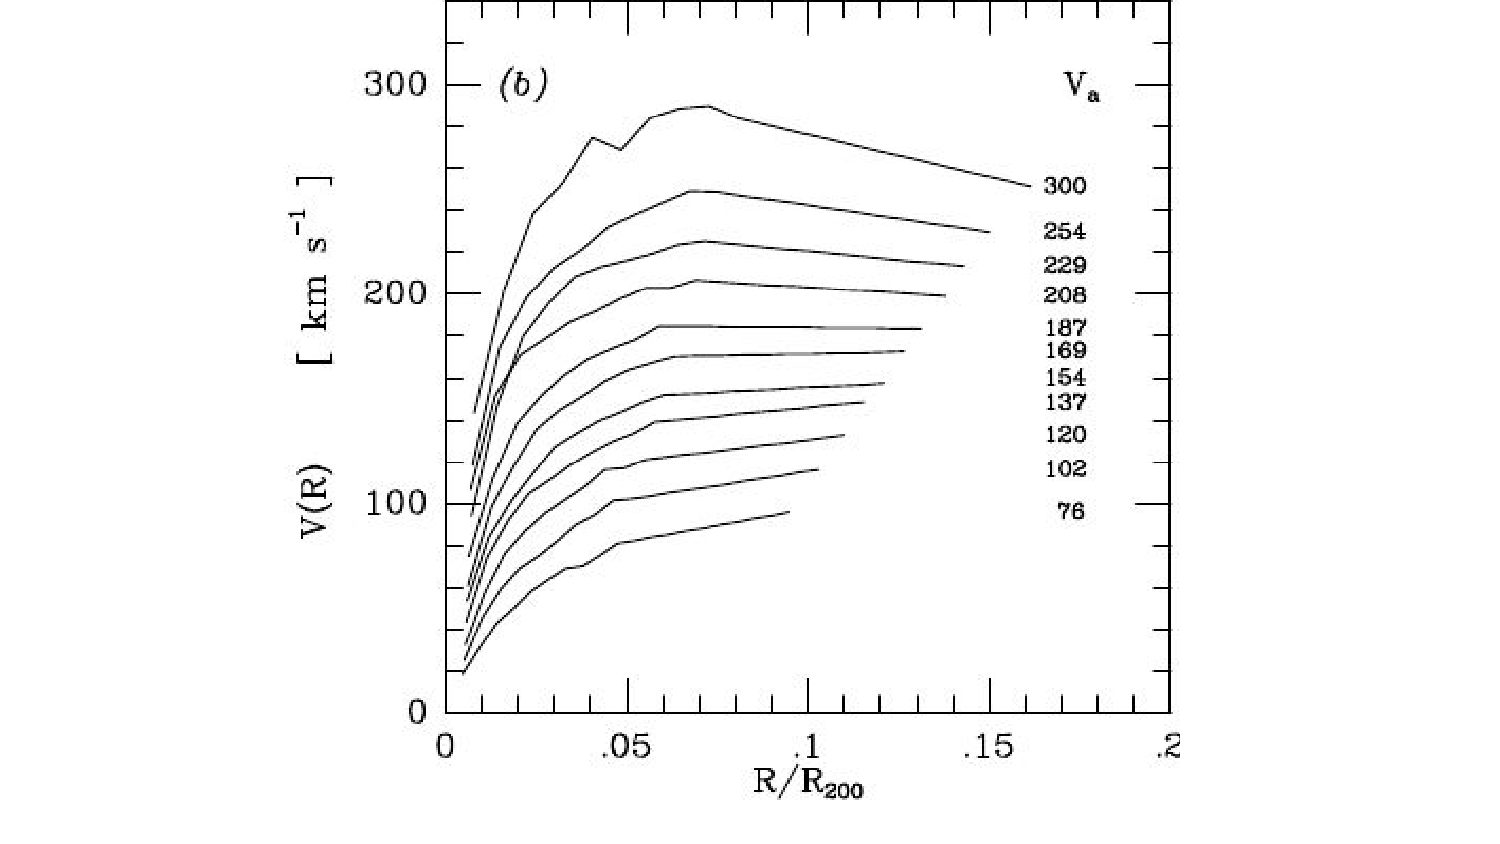
\includegraphics[width=\linewidth]{URC}
     \caption{\emph{Universal Rotation Curve spectrum, Used with permission from Ref.\citep{salucci}}}
     \label{fig:URC}
\end{figure}
  

  
    
 \begin{figure}[h!]
%\scalebox{0.25075}%
      \centering
      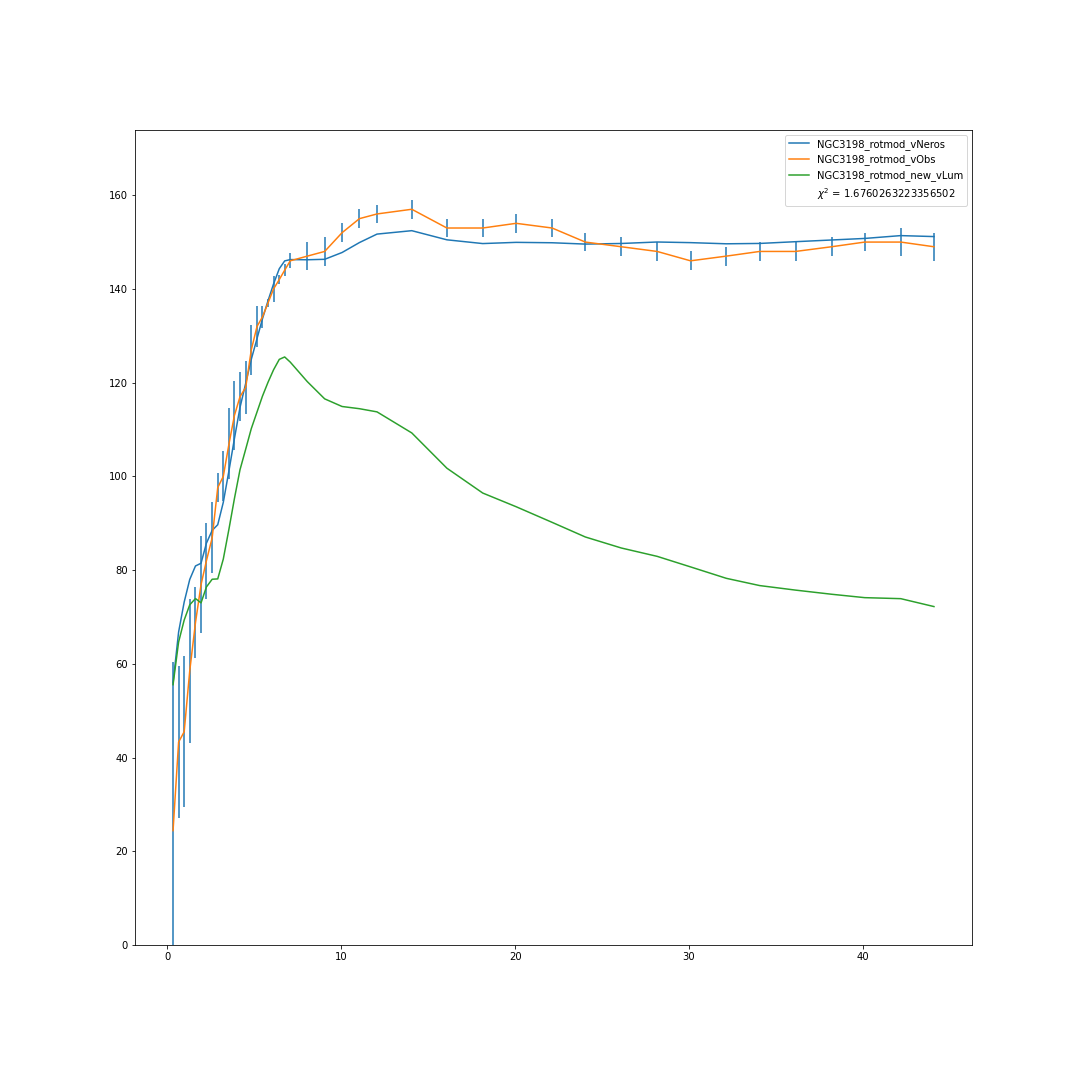
\includegraphics[width=\linewidth]{figures/NGC3198_rotmod_XueSofue.png}
      \caption{\emph{Rotation Curve of NGC 2403 \cite{Blok1}.   Rotation curve data blue dots with  error bars,  Keplerian velocity from luminous mass estimated by   green line,   RCFM fit blue line.} }
      \label{fig:NGC2403}
  \end{figure}
%%%%%%
%%%%%%%%
%%%%%%
%%%%%%%
%%%%%%
%%%%%%
\section{A New Rotation Curve Fitting Model   \label{sec:dos}}
 
 
 \subsection{old rotation curve fitting formula}
 
  

 The   dark matter rotation curve formula   is of the form

 \begin{equation}
v(r)^2_{obs}  =  v(r)^2_{lum}  +  v(r)^2_{dm},   
\label{eq:zonte1}
\end{equation} 

  where all velocities are assumed to be circular orbits, in the plane of the disk,  about the rotation axis of the galaxy at  $r=0$. 
Terms in  $v_{obs}$ are the velocity parameters  from a  Lorentz boost from the frame of the  Doppler shifted spectra $\omega'$
   

 \begin{equation}
 \frac{v_{obs} }{c}=
\frac{  \left( \frac{\omega'(r)}{\omega_o}\right)^2 -  \left( \frac{\omega_o}{\omega'(r)} \right)^2 }{  \left( \frac{\omega'(r)}{\omega_o}\right)^2  +  \left( \frac{\omega_o}{\omega'(r)}\right)^2 },
\label{eq:modelLumA}
\end{equation} 

 in flat Minkowski spacetime, to the 
  characteristic lab rest-frame frequency is $\omega_o$. Terms in $c$ are the constant vacuum light speed.  
  
  
 Terms in  $v_{lum}$ come from observations of total light  (photometry) interpreted by Population Synthesis Models (PSM) mass-to-light ratios as mass, consistent with Poisson's equation, and  hence orbital velocities  
  
   \begin{equation}
v(r)_{lum}^2 = \gamma_b v(r)_{bulge}^2 +  \gamma_d v(r)_{disk}^2 + v(r)_{gas}^2.    
\label{eq:zonte3}
\end{equation} 
  
 Terms in    $\gamma_i$  are the mass-to-light ratios for the stellar bulge $\gamma_b$ and disk $\gamma_d$ respectively, which come from PSM. Gas measurements do not require  a mass-to-light ratio due to different measurement techniques \citep{2016Lelli}.  
 Terms in $v^2_{dm}$ represent
the dark matter contribution to the dynamics, and is  the algebraic difference of the   terms  $v^2_{obs}-v^2_{lum}$. 

    Eq.~\ref{eq:zonte1} and Eq.~\ref{eq:zonte3} are quadratic velocity   sums to represent  sums of the  gradients in the gravitational potentials in radius, 
 for each mass contribution obeying the  central gravitational    force law   

\begin{equation}
 \frac{\partial \Phi(r)_{lum}}{\partial r}    =\frac{v(r)_{lum}^2}{r}.   
    \label{zoochance1}
\end{equation}

  
The   Newtonian gravitational potential is

\begin{equation}
      \Phi(r)  = -G \int d^3r'  \frac{ \rho(r') }{r-r'} ,
      \label{eq:Newt}
      \end{equation}

which solves Poisson's equation

\begin{equation}
\nabla^2 \Phi(r)_{lum}  = 4\pi G \rho(r)   
    \label{whatsgood}
\end{equation}

 for $G$  Newton's   gravitation constant, and 
$\rho(r')$  the mass density. 
  



\subsection{New Rotation Curve Fitting Formula}

 The  new 
frame-dependent Rotation Curve Fitting Model (RCFM) we propose relies on 
replacing the gradient in the potential    $v^2_{dm}/r$  attributed to   dark matter,  with  Lorentz-type transformations between galaxy frames.  This is the same term targeted by MOND in a subsequent evolution, RAR, to support the idea of a new acceleration scale, as this term is the gradient in the potential. 
 We  instead   assume terms from Doppler shifted spectra in $v^2_{obs}/r$ include both contributions from relative translation motion ($v^2_{lum}$) and from relative curvature (vis. relative galaxy imprints). 
 Like MOND, We assume baryonic mass is the only mass in this problem.
 
We emphasize,  luminosity   is a Lorentz scalar, therefore invariant under the assumption of a good distance estimate, and   a faithful tracer of baryonic mass, and that    the observed   
   Doppler shifted spectra is part  a Lorentz 4-vector, and so    must transform in a Lorentz sense. 
In addition, we will 
   guess  heuristically that shifts in   spectra   due to relative velocity and relative acceleration are separable \cite{Jack,Cisn}, perhaps roughly  as in Eq.~\ref{eq:zonte1}.
  In what follows, all   terms  can be assumed to  be functions of radius except the model's free parameter $\alpha$,  which is single valued for each galaxy fitted, and the speed of light $c$.  Further, we will assume that the small deviations from flatness represented by spiral  galaxies are important in interpreting Doppler shifted spectra. 
   
   The new rotation curve fitting model (RCFM) we propose  is
   

\begin{equation}
v_{rc}^2 =  v_{lum}^2+\alpha \kappa^2 v_{1} v_{2},  
\label{eq:zonteLCM}
\end{equation}  

for $\alpha$  the free parameter,  
$\kappa$  a curvature ratio 

 \begin{equation}
\kappa=\frac{\Phi_{gal}}{\Phi_{mw}}, 
\label{eq:kappa2}  
\end{equation}  

 and $\Phi_{gal}$ the    Newtonian gravitational potential of the galaxy being observed, and $\Phi_{mw}$ that of  the Milky Way, to be compared one-to-one in radii. 


 Terms in $v_1$   are   
 
   \begin{equation}
       v_1 = \sinh \zeta. 
   \end{equation}
 
 for a rapidity angle $\zeta$ defined by the    Lorentz exponential  term  
  
   
     \begin{equation}
     e^{\zeta}=  \frac{\omega_{mw}}{\omega_{gal}}  =\sqrt{\frac{g_{tt}|_{gal}}{g_{tt}|_{mw}}},
      \label{eq:gravRS}
    \end{equation}
    
 for  clock terms $g_{tt}$   defined in the   weak field Schwarzschild limit  \cite{Hartle} as, 
 
  \begin{equation}
      g_{tt}= -( 1 - 2\Phi/ c^2).
      \label{clocktime}
  \end{equation} 
  

Terms in $v_2$ are 

\begin{equation}
v_{2} =  \cosh \tau, 
\label{eq:hyperbolico}
\end{equation}


 
 
  for a rapidity angle $\tau$ defined by the    Lorentz exponential  term  
  
 
\begin{equation}
    e^{\tau}=   e^{(\zeta+\eta)/2},
\end{equation}
 
for the  flat field-frame
Lorentz exponential  

\begin{equation}
    e^{\eta}=\frac{\omega_{l}}{\omega_o}= \sqrt{\frac{1+\beta}{1-\beta}}.
    \label{eq:flat}
\end{equation}  
     
Terms in 
$\beta = v_{lum}/c$ are the
Keplerian rotation velocities  estimated from total light  $v_{lum}$, and  associated with  frequency shifts $\omega_{l}$      by a Lorentz boost   

 \begin{equation}
 \frac{v_{lum} }{c}=
\frac{  \left( \frac{\omega_{l}}{\omega_o}\right)^2 -  \left( \frac{\omega_o}{\omega_{l}} \right)^2 }{  \left( \frac{\omega_{l}}{\omega_o}\right)^2  +  \left( \frac{\omega_o}{\omega_{l}}\right)^2 }. 
\label{eq:lumlorentz}
\end{equation} 
 
 
  
 
 
The   term $v_1$ maps the gravitational frame of the observed galaxy into that of the Milky Way. The   term $v_2$    maps from  the   curved 2-frame  of  Eq.~\ref{eq:gravRS},  to  the flat 2-frame where we make observations. 
  That this second transformation  is necessary is evidenced by the local constancy of the speed of light. 
By use of Eq.~\ref{eq:flat}, we are  asserting  that Keplerian rotation curves are     the best estimate of flatness, since dark matter is not required to  reproduce the rotation curve of our Solar System.
 
    
  
 
 Note, when viewed as    Rindler's accelerated coordinates\cite{MTW,Wald, rindler2013essential}, the   $v_1$ term is  timelike   and $v_2$ is spacelike. The  $v_1$ and $v_2$ functions reported here have been   selected based on goodness of fit, for tests of various hyperbolic functions  explored in   \cite{Cisneros:2013vha,Cisneros:2014fea,Cisneros2015,Cisn2016}. 
 The    functions 
 reported here fit the galaxies in the SPARC sample twice as well as the previous functions,  and twice as well as MOND fits to the same, as judged  by comparison of the  average reduced $\chi^{2}$ values. 
 
  
 
%%%%%%
%%%%%%%
%%%%%%
%%%%%%%  
%%%%%%
%%%%%%%  
\subsection{Gravity Details \label{sec:gravDets}}

  
    
    
Lorentz exponential terms (Eq.~\ref{eq:gravRS} and Eq.~\ref{eq:flat})
  are    identified  as the field frame relationships defining the $v_1$ and $v_2$ transformations. We arrive at this result  by  comparison of 
     the  Lorentz transformation in  Eq.~\ref{eq:modelLumA} with 
 that of the    hyperbolic form \cite{rindler2013essential} 


     \begin{equation}
         \frac{v}{c} = \tanh \theta = \frac{e^\theta - e^{-\theta}}{e^\theta + e^{-\theta}} .   
         \label{boost}
     \end{equation} 

 
 
 
 
 
Lorentz exponential terms in  $v_1$ and $v_2$ are parametrized with ratios of  the    Schwarzschild gravitational redshifts

\begin{equation}
       \frac{\omega_1}{\omega_2}  =\sqrt{\frac{g_{tt}|_{P2}}{g_{tt}|_{P1}}} =\sqrt{\frac{|\xi^t\xi_{t}|_{P2}}{|\xi^t\xi_{t}|_{P1}}}.
      \label{eq:grav}
    \end{equation} 
    
    This formula is    intended to represent the changes in a photon frequency moving from point $P1$ to $P2$,  in the same manifold. 
To extend this relationship Eq.~\ref{eq:grav} to connect 
  two distinct gravitational manifolds,  we    note that Eq.~\ref{eq:grav} came from  the conservation properties of  the timelike  Killing vector fields  
   $\xi^t(r)$  \cite{Wald}.   
   To relate two such manifolds using Eq.~\ref{eq:grav}, we consider the that 
 the  timelike Killing fields rely on  the
  $g_{tt}(r)$, 
  which are in  turn   parametrized by  the Newtonian  gravitational potentials about the galaxy center Eq.~\ref{clocktime}. 
  
 
   
 Usually, gravitational potentials of galaxies are compared and calculated in  a globally flat background spacetime, where at the large $r$ limit, the potential $\Phi$ is required  to go to zero. 
 In calculations, this amounts to integrating the potential from the outside to the inside, from zero potential at the large  $r \to \infty$ limit, to a negative maxima at   $r\approx 0$. 
This procedure  ensures   energy goes to zero at infinity, which is consistent with a picture of a globally flat embedding space.   However, since 
  the external environments of galaxies at the large $r$  limit of the data appear to be  extremely complicated  and diverse  \cite{Pomarede:2020pme,Hoffman:2017ako},   we 
  note that  galaxies cannot be compared to each other at this limit in any meaningful way.

  Wolfgang Rindler said,        ``the center of each galaxy provides a basic local standard of nonacceleration ... so then can be treated like a local inertial frame relative to its own center.''\cite{rindler2013essential}. To relate two such manifolds then, will rely upon synchronizing the galaxy centers. 
  What we do know is that galaxy centers can be compared inertially and that the Killing fields at the event horizon are all the same, namely their norm gives $g_{tt} = 0$. 
 So,  to synchronize galaxies and Killing fields, we   integrate the gravitational potentials from the small $r$ limit to the extent of the data in $r$. This means we are comparing all galaxies from the place we know that their clocks are all set to zero, hence they can be compared inertially by Lorentz-type transformations. 
   

 \begin{equation}
    | \Phi | = \left|  \int^{R-big}_{r-small} \vec{F_r}\cdot\vec{dr}\right|.
      \label{eq:Newt2}
      \end{equation}
 
 

   
 Potentials calculated in this way still obey the central force law for test particles moving in circular orbits in Eq.~\ref{zoochance1} and Poisson's equation Eq.~\ref{whatsgood}.
   
 

%%%%%%
%%%%%%%
%%%%%%
%%%%%%%
 
 %We   assume   the  additional symmetry of the  Tetrad-formalism \cite{BertschingerClassTetrads}, which attaches  a    local Lorentz frame   at each point in the manifold 
   % \begin{equation}
      %  g^{\mu \nu} = \eta^{\alpha \beta} e^\mu_\alpha  e^\nu_\beta
   % \end{equation} 
    
  %  so that the orthonormal  basis vectors  $e^\mu_\alpha$ carry the information of the physical spacetime, and the tetrad at each point is Lorentzian and   can endure 3 boosts and 3 rotations \cite{BertschingerClassTetrads}.  
% 
%-  WALD - the basis is the $e^\mu$ and these are $\sqrt{g_{tt}}$ so they not flat, but inner product of one of those bad boys with the inverse covector of the other galaxy, would give us eq. 10, also checkiyo if the indices are correct, originally had a, b lower indices on the basis. CHECK) 
%%%%%%
%%%%%%
%%%%%%% 
%%%%%%
%%%%%%
%%%%%%%  
%%%%%%
%%%%%%%  
%%%%%%
%%%%%%%
\section{Data \label{sec:data}}
 
 \subsection{SPARC }
 We fit the SPARC dataset  of  174 nearby galaxies with extended rotation curves from atomic hydrogen (HI)  and H-$\alpha$ (Spitzer Photometry and Accurate Rotation Curves)\cite{2016Lelli}. HI provides the most reliable
 rotation curves because it is dynamically cold, traces circular orbits, and can be observed several effective radii past the stellar disk. This sample of rotationally supported galaxies   spans the widest range of masses and morphologies currently available. In addition, these galaxies are  accompanied by luminous mass models which come from   Spitzer Photometry in the 
   near infrared  at 3.5$\mu m$, which is widely believed to be the best tracer of stellar mass   in population synthesis models and   gives mass-to-light (M/L) ratios which are almost constant, independent of star formation history \cite{BelldYong,10.1093/mnras/sty3223}.  Stellar M/L ratios   translate   photometry to dynamics. 
   
   
     All terms in $\Phi(r)$ used in this paper  are    integrated from estimates of the baryonic mass, reported kinematically as in Eq.~\ref{eq:zonte3} in the      SPARC  library.   These velocities  are constructed from photometric observations of surface brightnesses, interpreted   by a Population Synthesis Model (PSM)\cite{10.1093/mnras/sty3223} as     masses. 
PSM rely upon a complex  suite of  assumptions regarding galaxy evolution, metallicities and initial mass functions  \cite{BelldYong,10.1093/mnras/sty3223}. PSM predict   mass-to-light ratios  $\gamma_i$
 which translate  luminosity into mass dynamics as in Eq.~\ref{eq:zonte3}. 
     The $v_{disk}$ and $v_{bulge}$ are reported in the SPARC database with $ M/L = 1$ in units of  $M_{\odot} / L_{\odot}$   at 3.5$\mu m$.
     Gas fractions $v_{gas}$ are calculated from surface density profiles of HI  with the formalism given in  \cite{1983MNRAS.203..735C} and scaled 
     a factor 1.33 to account for cosmological helium abundances.  
     Contributions from molecular gas are ignored   because CO data are not available for most SPARC galaxies. 
     Error on these velocities is estimated at $20\%$ \cite{2016Lelli}. 
     
      
  
 

  
%ASK STACY: they use M/L =1, so why he say mines are high? 
   %but also says in Lelli 2016 paper they use 0.5\gamma for M/L
 %Their final science sample is made of 153 galaxies.
 


%%%%%%
%%%%%%
%%%%%%%
\subsection{Milky Way}
%''Mapping the Milky Way is one of the key science drivers for LSST.''~Mario Juric ,  UW
The rotation curve fitting model presented here requires a static choice for the baryon distribution of the   Milky Way (MW).   Mass-modeling of the MW is an under-constrained problem, due to     observing from       within  the system  \cite{1991ARA&A..29..409F}.
 Outside of our position at 8 kpc in the disk of the MW, the data is very 
 noisy, see  Fig.~\ref{fig:mwSofue}. This is the central way in which this model can be falsified, if dark matter is found to be required to reproduce the rotation curve of the MIlky Way from independent tracers Mario Juric, etal. 
 
 \begin{figure}
    \centering
    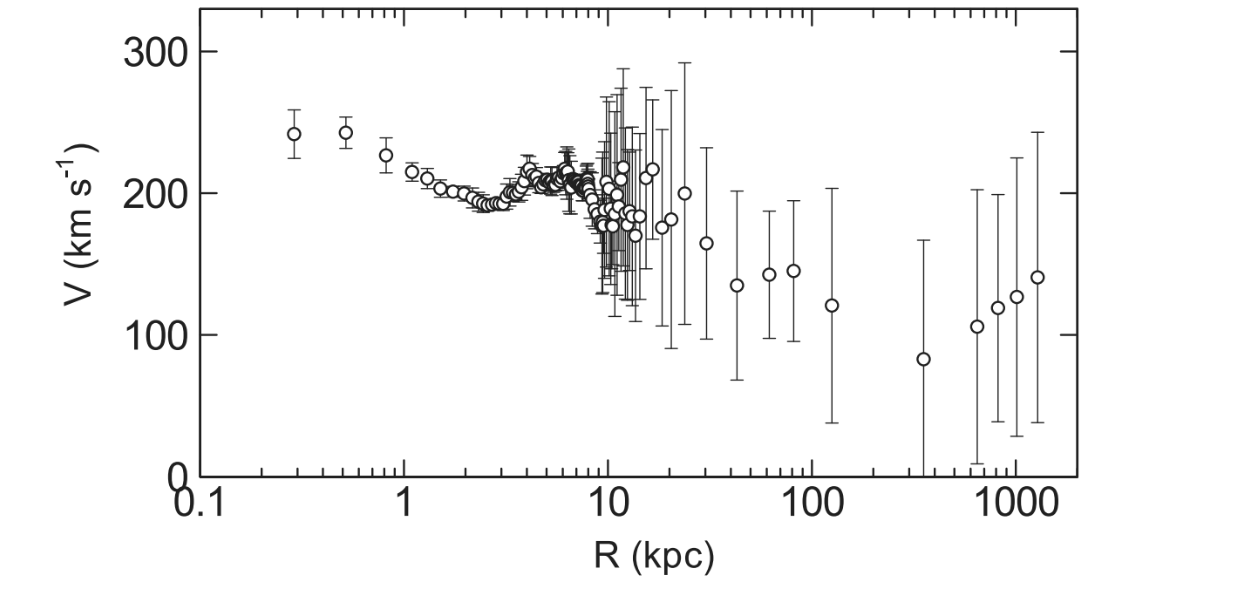
\includegraphics[width=\linewidth]{Sofue_MWtoLGData}
    \caption{Milky Way rotation curve data from radio signals and SDSS CO star line shifts  \cite{Sof11}}
    \label{fig:mwSofue}
\end{figure}

%Sofue: We included the circular velocities from an SDSS blue stars analysis by Xue et al. (2008; their model 1) by correcting for a systematic difference in the veloc-ities of about 20 km s1, due to our V0 = 200 km s1 instead of their 220 km s1.
%ugggh. have to look at the first two papers to see what assumptions they make. 
%We decomposed the newest rotation curve into a de Vaucouleurs bulge, an exponential disk, and an isothermal dark halo (Sofue et al. 2009).
%OBS METHOD: 
%An inner rotation curve was obtained by a terminal-velocity method applied to radio line observations
% An outer rotation curve was obtained by combining the CO star line velocities and the optical distances
%and by the HI disk-thickness method
%de Vaucouleurs bulge of mass Mb = 1.8 1010 Mˇ with a scale radius of Rb = 0.5 kpc, an exponential disk of mass Md = 71010Mˇ with a scale radius of Rd = 3.5 kpc,
%In the inner Galaxy at R .10 kpc, the rotation velocity is predominantly determined by the bulge and disk contributions, and R < 0.5 kpc it is almost determined by the bulge alone.


  We test the RCFM against two MW models;  a hybrid model from \citet{Xue} and \citet{Sofue}, a model from Stacy McGaugh  as summarized in Table ~\ref{tab:my_label}.
  
%   \begin{table*}[h!]
%      \centering
%      \begin{tabular}{|c|c|c|}
%      \hline
%        Author & Position of the Solar system   &  scalelength disk\\
%        \hline
%        Sofue \cite{sofue2009unified,10.1093/pasj/61.2.153,Sof11}   & 8 kpc &\\
%             \hline
%        McGaugh\cite{2021DDA....5240103M} & &\\
%         \hline
%        Klypin&&\\
 %        \hline
%        Enbang Li&&\\
%         \hline
%      \end{tabular}
%      \caption{MW}
%      \label{tab:my_label}
%  \end{table*}
  
 

 


 








\section{Fit Analysis and Constraining the free parameter \label{sec:analysis}}
 
 
In RCFM fits reported here, the    bulge and disk mass-to-light ratios are allowed to vary freely from an initial value of $1.0$ (See Eq.~\ref{eq:zonte3}). The resulting average mass-to-light    values are within stated criteria    of $\pm 20\%$ \cite{2016Lelli}. The gas fractions (HI scaled for Helium abundance) are fixed,  though addition of molecular gas could increase mass fractions in the inner kiloparsec of a galaxy   \cite{2004ApJ...609..652M}.

\subsection{Fitting galaxies}
\emph{We'll want a better title, and this is basically a first draft.  Also, this probably isn't the right order to do things in. Maybe we should first address which galaxies we analyze, then the actual fitting, then interpreting $\alpha?$}

The equations outlined in Section \ref{sec:dos} contain three free parameters that must be determined for each galaxy: the model free parameter $\alpha$ and the mass-to-light ratios for the stellar bulge and disk, $\gamma_b$ and $\gamma_d$ respectively. To compute these values, a fitting procedure is followed.

Data for a Milky Way model is read in, giving $v_{lum}(r)$ for a series of measurement radii in the Milky Way. The galactic potential is computed as per Eq.~\ref{zoochance1} by numerically integrating

\begin{equation}
\Phi(r) = \int_{inner}^{outer} dr \frac{ 
v(r)^2_{lum} 
}{r}
\end{equation}

The data for other galaxies contains several pieces of information: the orbital velocities $v_{obs}(r)$ from Doppler shifted spectra, the uncertainty on that measurement $v_{err}(r)$, and the components of the luminous mass interpreted as orbital velocities,  $v_{bulge}$, $v_{disk}$, and $v_{gas}$. 

For the fitting process, $v_{lum}(r)$ is computed for the galaxy as per Eq.~\ref{eq:zonte3}, based on given values of $\gamma_b$ and $\gamma_d$ (these are varied in the fit). The $\Phi_{gal}(r)$ associated with that galaxy is computed as above.

These two $\Phi$s are used to compute the components of the model. However, these components must be computed using matching values of $r$. To match radii, the $\Phi_{MW}(r)$ is interpolated and $\Phi_{MW}(r_{gal})$ is computed at the radii where there are observations in the target galaxy. Any point with a radius larger than the largest radius in the Milky Way model is discarded.

The terms in Eq.~\ref{eq:zonteLCM} are calculated as follows, to calculate the  $v_{rc}$ that can be fitted to the   $v_{obs}$. 

$\kappa(r)$ is simply computed as in Eq.~\ref{eq:kappa2} by diving the two potentials at each radius.

To calculate $v_1$ and $v_2$,   the terms $e^\zeta$ and $e^\eta$ are needed, which we rename for convenience. These are as defined in equations (REF) and (REF)

\begin{equation}
    \psi_{curve}(r) = e^\zeta = \sqrt{\frac{1 - 2\Phi_{gal}(r)}{1 - 2\Phi_{MW}(r)}}
\end{equation}

\begin{equation}
    \psi_{flat}(r) = e^\eta = \sqrt{\frac{1 + \beta_{gal}(r)}{1 - \beta_{gal}(r)}}
\end{equation}

Where

\begin{equation}
    \beta_{gal}(r) = \frac{v_{lum,gal}(r)}{c}
\end{equation}

Then the $v_1$ and $v_2$ terms are the respective hyperbolic functions.

\begin{equation}
    v_1(r) = \sinh(\eta) = \frac{\psi_{curve}^2(r) - 1}{2 \psi_{curve}(r)}
\end{equation}

\begin{equation}
    v_2(r) = \cosh((\zeta + \eta)/2) = \frac{\psi_{curve}(r) \psi_{flat}(r) + 1}{
    2\sqrt{\psi_{curve}(r) \psi_{flat}(r)}}
\end{equation}

These are assembled as in equation \ref{eq:zonteLCM}, along with $\alpha$ of a given value, to get a predicted $v_{rc}$. The $\chi^2$ of this $v_{rc}$ vs $v_{obs}$ is minimized by varying the three free parameters using the {\tt scipy.optimize.curve\_fit} utility in Python.

\subsection{Evaluating Goodness-of-fits and Comparing Milky Way Models}
The $\chi^{2}$ values for fits shown in Table II are remarkably low, providing confidence in the faithfulness of fits to data. The functional form of ${v_1}$ and ${v_2}$, the mapped velocities used in fits, had a major effect on $\chi^{2}$ of fits to the training set. The ${v_1}$ and ${v_2}$ functions chosen for use in our model resulted in the lowest $\chi^{2}$ and thus provided fits that described the data with the most accuracy according to that metric.

The residuals of fits using different Milky Way models (McGaugh, XueSofue, Juric?) were compared to determine which resulted in the best fits. The different Milky Way models vary in their underlying assumptions about the fundamental structure and gravitational behavior of the Milky Way. For example, McGaugh [cite] assumes a galactic bar at the center and thus does not include velocity data of the inner 5 kpc of the Milky Way. Differences in assumptions in the Milky Way affected the fits produced by the model by changing the values of the Milky Way's gravitational potential and angular velocity used in calculations, as described in Equations 8 and 10. 

Histograms of residuals normalized by subtracting the mean and dividing by the standard deviation are shown in figure 5. In all cases, residuals of model fits to observed velocity data followed a narrow distribution centered at zero, albeit with heavy tails. The behavior of the residuals did not vary greatly between Milky Way models, suggesting that the fitting parameters in our model are flexible and can be used to provide accurate fits across different Milky Way model assumptions. A Gaussian fit on residuals from fits using the McGaugh Milky Way models gave a mean of 0.024 kpc, standard deviation of 2.786 kpc and a full-width half-maximum (FWHM) of 6.561 kpc, whereas a Guassian fit to the residuals from fits using the XueSofue Milky Way models gave a mean of -0.067 kpc, standard deviation of 3.578 kpc and a FWHM of  8.426 kpc. The small values associated with these quantities in both cases provide confidence that our fits matched data closely, even with outliers included. Notably, fits using the McGaugh Milky way model agreed slightly more with observations, resulting in a distribution of residuals with a smaller mean, standard deviation, and FWHM when fit to a Gaussian distribution.
\begin{figure}[h]
     \centering
     \begin{subfigure}[b]{0.475\textwidth}
         \centering
         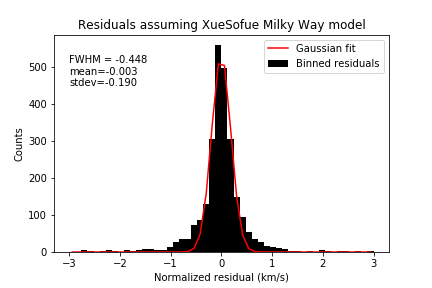
\includegraphics[width=.8\linewidth]{figures/ResidualHist_GaussFit_v1_sinh_v2_cosh.png}
         \label{fig:XueSofue residuals gaussian fit}
     \end{subfigure}
     \begin{subfigure}[b]{0.475\textwidth}
         \centering
         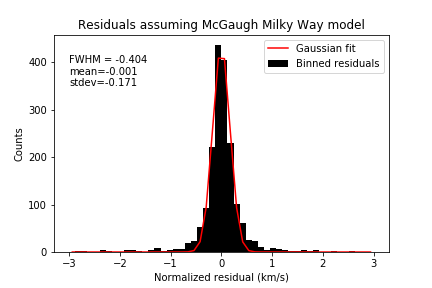
\includegraphics[width=.8\linewidth]{figures/ResidualHist_GaussFit_v1_sinh_v2_cosh_McGaugh.png}
         \label{fig:McGaugh residuals gaussian fit}
     \end{subfigure}
     \begin{subfigure}[b]{0.475\textwidth}
         \centering
         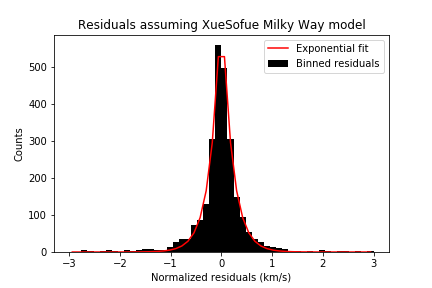
\includegraphics[width=.8\linewidth]{figures/ResidualHist_ExpFit_v1_sinh_v2_cosh.png}
         \label{fig:XueSofue residuals exponential fit}
     \end{subfigure}
     \begin{subfigure}[b]{0.475\textwidth}
         \centering
         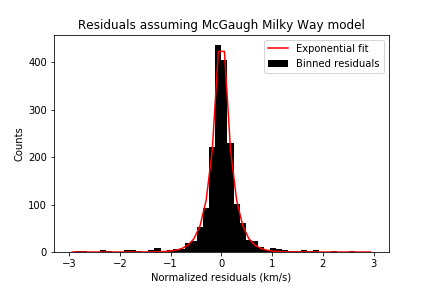
\includegraphics[width=.8\linewidth]{figures/ResidualHist_ExpFit_v1_sinh_v2_cosh_McGaugh.png}
         \label{fig:McGaugh residuals exponential fit}
     \end{subfigure}
        \caption{Normalized residuals from fits assuming either XueSofue of McGaugh Milky Way models, fitted to a Gaussian or exponential function. The exponential fit captures peak and tails in residuals better than the Gaussian fit.}
        \label{fig:residual graphs}
\end{figure}
Yet, the Gaussian fits did not quite capture the full peak and heavy tails in the residuals. This suggests that there may be systematic error in the data, possibly resulting in the fact that the error in the observed velocities is not Gaussian. (Analysis of underlying data error and if there are any trends in tails add here soon) To address this, the residuals were also fit to an exponential function shown in figure 5. The exponential function captured both the peak and the heavy-tailed behavior of the distributions more faithfully.

%\subsection{NGC 3198 and other galaxies(UNDER CONSTRUCTION)}\cite{1985ApJAlbada} studies this galaxy, which MOND has troubles with. This galaxy has   a thin exponential disk (de Vaucouleurs 1959),(Freeman 1970).  \cite{Toky} mentions that MOND fails to fit NGC 3109, which we fit exceedingly well ($\chi^2 = 0.32$).NGC 2841 is also a problem for MOND
%%%%%%
%%%%%%%%
%%%%%%
%%%%%%%
%%%%%%

 
\subsection{Population synthesis Models, Geometry  and  Mass-to-light ratio results}

 
  
    It is commonly assumed when making a population synthesis model, to produce  mass-to-light ratios $\gamma$ for  stellar disks and  bulges from observations of total light,  that   the stellar bulge and gas halo  are spherically symmetric and   the stellar disk is axially symmetric \cite{1954AJ.....59..273S}.
    In exhaustive studies,    \citet{McGaugh2016RAR} have shown the most likely values for the mass-to-light ratios for all morphological types of galaxies are 
    $\gamma_{[3.6]} = 0.7 M_\odot/L$ for bulges  and $\gamma_{[3.6]}= 0.50 M/L [25]$ for disks. 


    
 The assumption of spherical symmetry is common  in evaluation of the   rotation curve velocities from integrated potentials \cite{2022A&A...664A..40M,PhysRevD.70.083509}, because numerical integration of the disk is  computationally intensive, and requires assumptions of  boundary conditions,   relevant physical scales,  etc. which adds extra free parameters \cite{2011A&A...531A..36H}.
Use of the spherical  symmetry assumption
    in the inner region of a galaxy $r< R_e/3$, where $R_e$ is the exponential scale-length of the disk,  overestimates the potential of a thin disk by $\approx 50\%$,  but maintains the same descending line shape\cite{Chatterjee}. We use the spherical assumption in RCFM calculations, since  the 
 Schwarzschild metric is spherically symmetric.     As can be seen in Table~\ref{table:M2L}, the RCFM fit results for average $\gamma$ across the SPARC sample   ( .561 disk (scaled down by factor of 2)  and 0.81 bulge) and for the  
the MOND/RAR results (disk 0.638 and bulge 0.733 ) are consistent within the $20\%$ error budget on luminous mass introduced in \cite{2016Lelli}.   
    
    
    
    
    Since  gravitational potentials converge for spherical and cylindrical geometries at the length of $r>R_e/3$,  where dark matter becomes important (see Fig.~\ref{fig:my_geom}), and because,   as noted in   \cite{McGaugh2016RAR},   
        adopting different mass-to-light ratios only
affects details, not the basic results, we keep this simplifying technique.    Furthermore, since  this is the region where dark matter is not required to reproduce the rotation curve \cite{1985ApJAlbada},   the computational benefits   outweighs the geometric differences.  
 Elsewhere it has been noted that the majority of introduced  error comes from uncertainties in the M/L ratios, rather than the geometry assumptions \cite{2016Lelli}. 
 
 
\begin{figure}
    \centering
     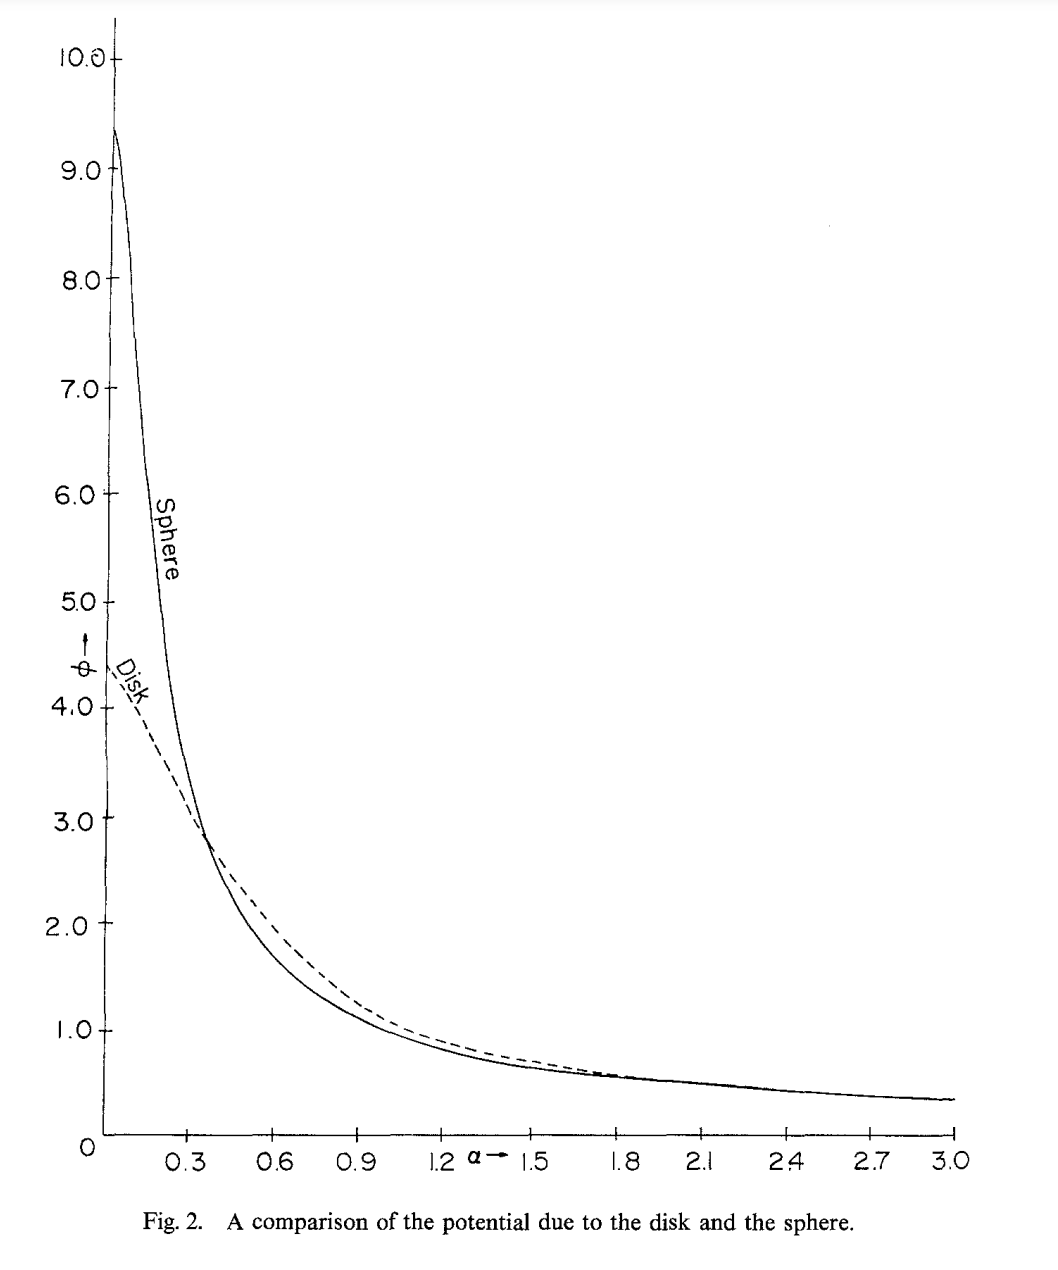
\includegraphics[width=\linewidth]{Chatterjee_SphereDisk.png}
    \caption{ $\alpha = r/R$, for $R$ the radial extent of the stars \cite{Chatterjee}}
    \label{fig:my_geom}
\end{figure}

\begin{figure*}[ht] 
  \begin{subfigure}[b]{0.5\linewidth}
    \centering
    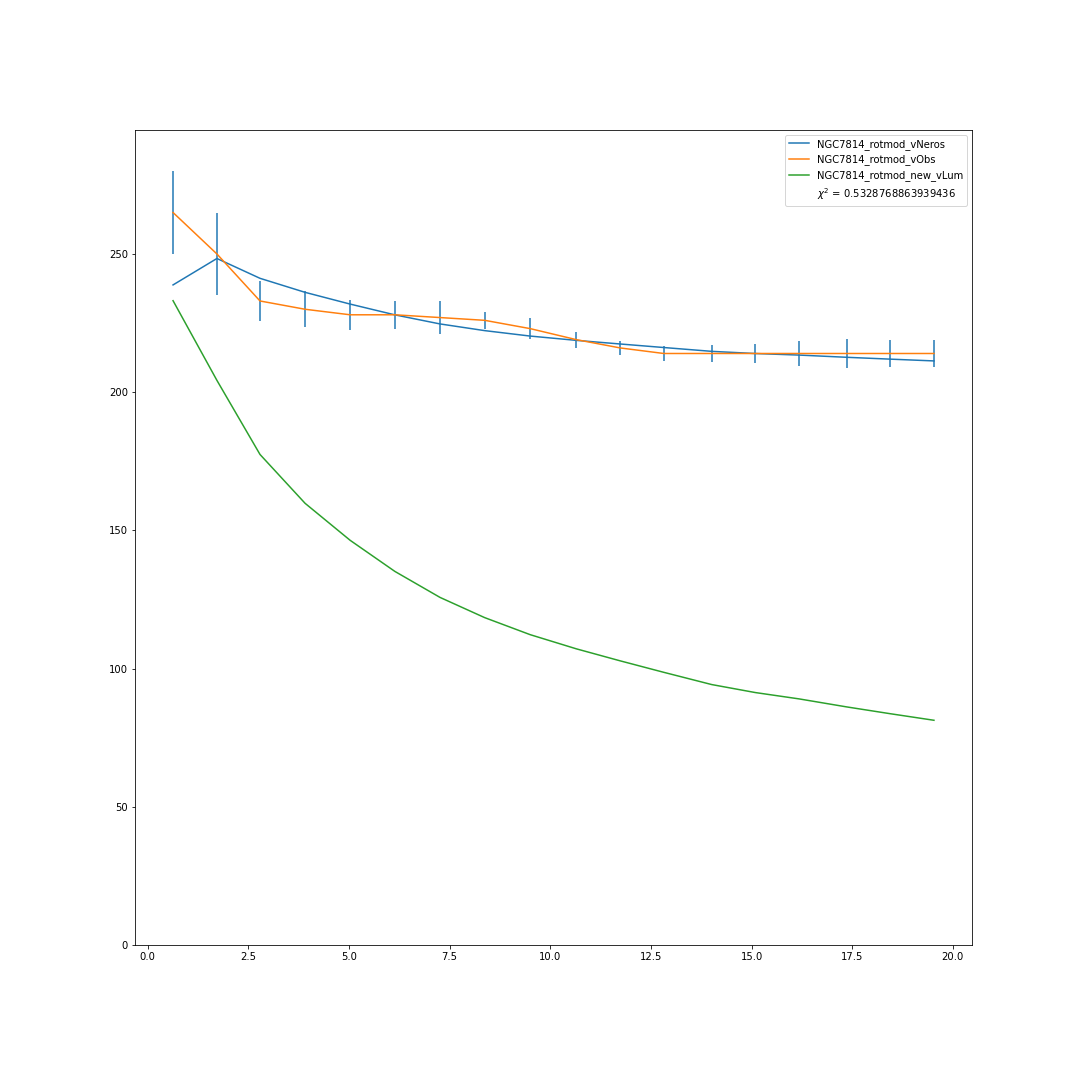
\includegraphics[width=0.75\linewidth]{figures/NGC7814_rotmod_XueSofue.png} 
    \caption{Bulge dominated NGC 7814} 
    \label{fig7:a} 
    \vspace{4ex}
  \end{subfigure}%% 
  \begin{subfigure}[b]{0.5\linewidth}
    \centering
    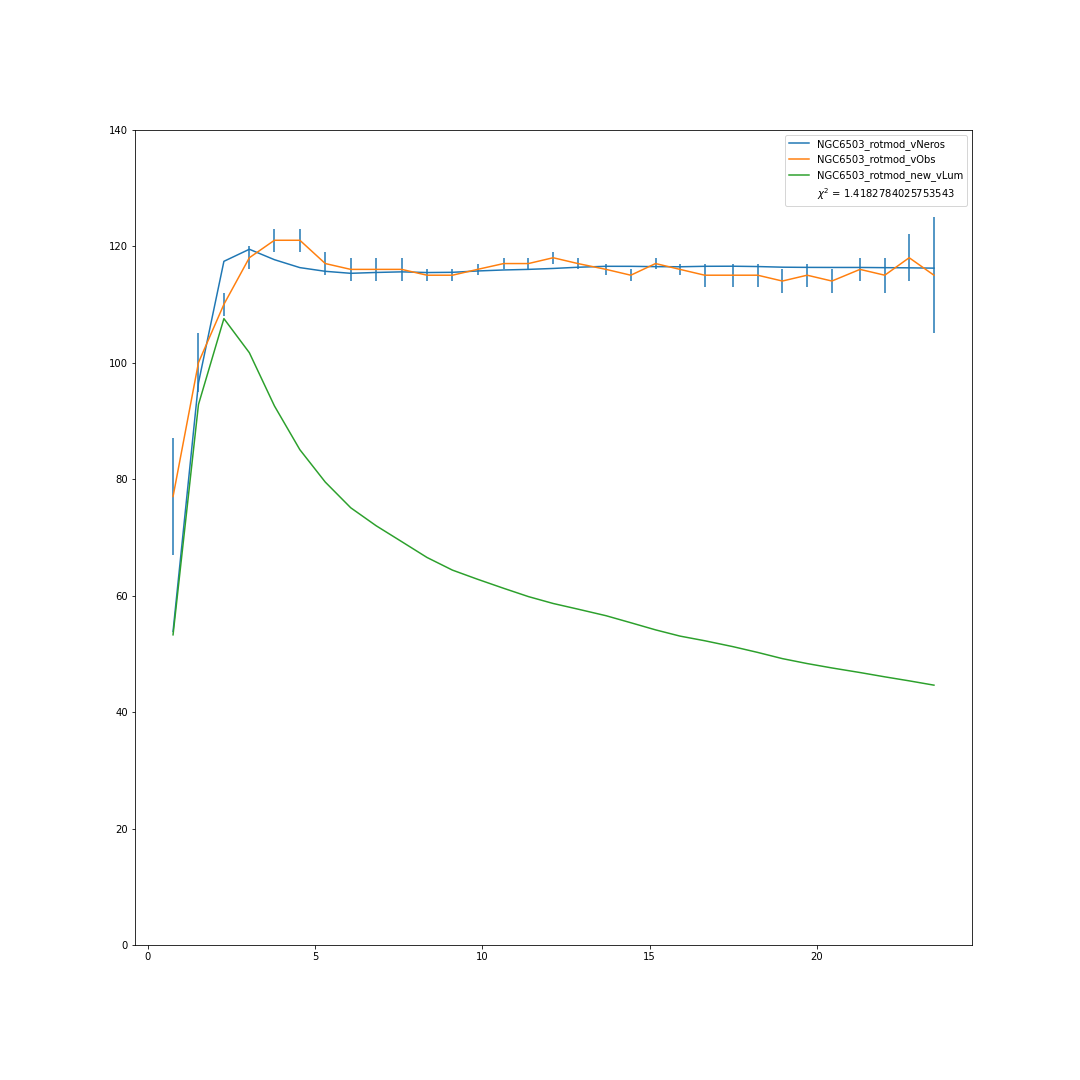
\includegraphics[width=0.75\linewidth]{figures/NGC6503_rotmod_XueSofue.png} 
    \caption{Disk dominated NGC 6503} 
    \label{fig7:b} 
    \vspace{4ex}
  \end{subfigure} 
    \begin{subfigure}[c]{0.5\linewidth}
    \centering
    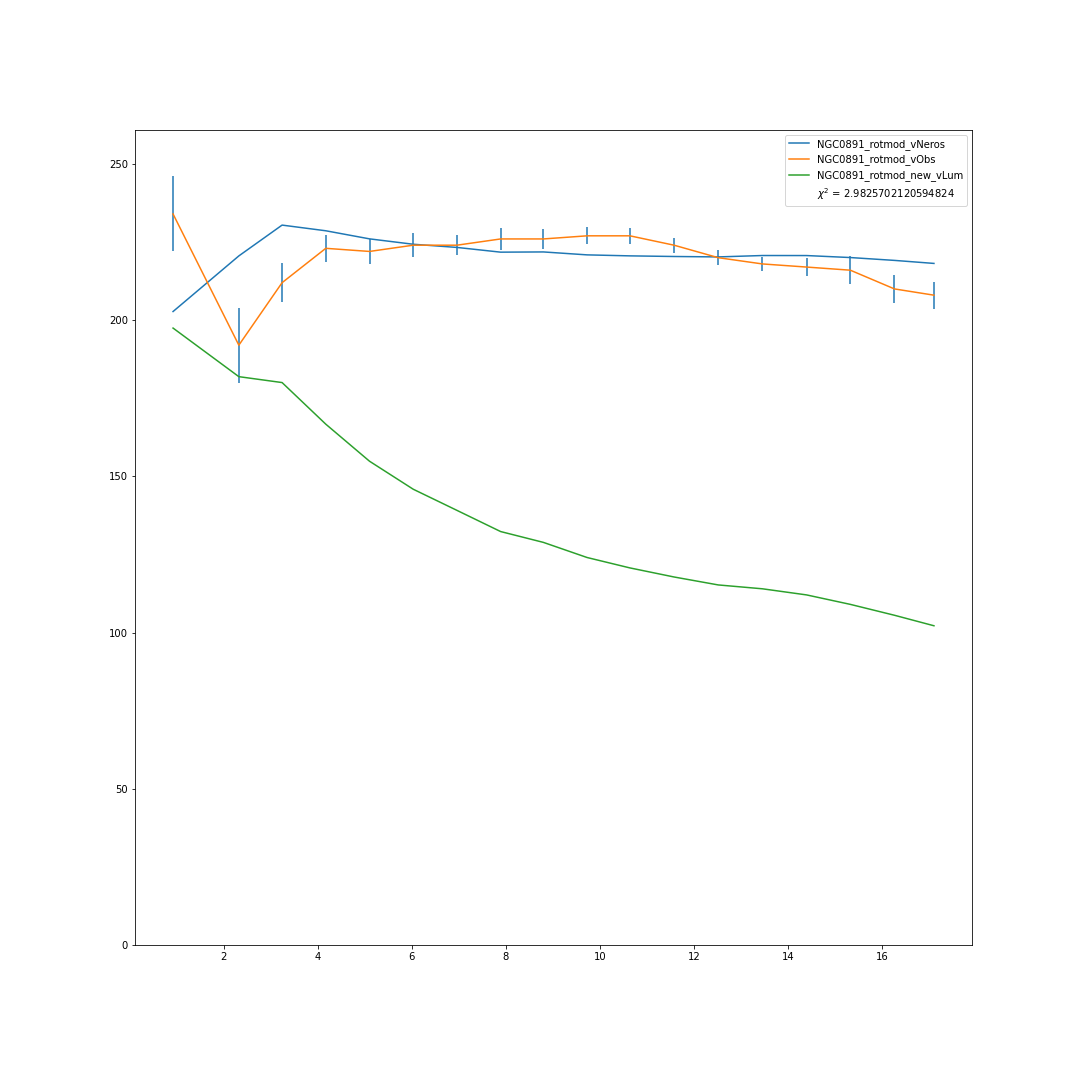
\includegraphics[width=0.75\linewidth]{figures/NGC0891_rotmod_XueSofue.png} 
    \caption{Disk dominated NGC 891} 
    \label{fig7:c} 
  \end{subfigure}%%
  \begin{subfigure}[c]{0.5\linewidth}
    \centering
    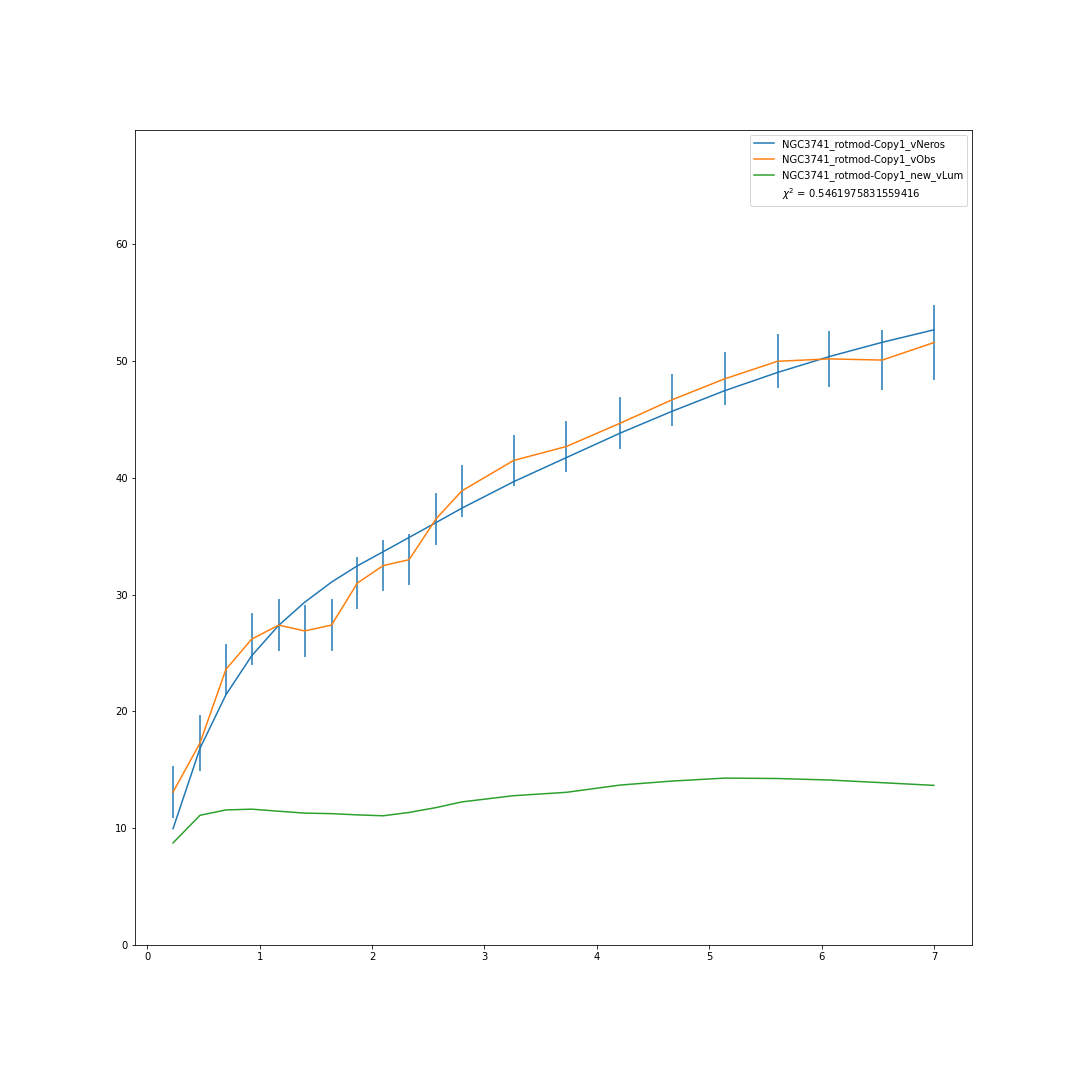
\includegraphics[width=0.75\linewidth]{figures/NGC3741_rotmod-Copy1_XueSofue.png} 
    \caption{Gas dominated NGC 3741} 
    \label{fig7:c} 
  \end{subfigure}%%
  \caption{Examples of range of spiral galaxy densities and RCFM rotation curve fits, points with error bars are the rotation curve data, Combined baryonic models are represented by the green lines, and the RCFM fit is the blue line. (MARCUS PAZ : NOTE: remove orange lines, fit through data distracts from our fit)  }
  \label{fig7} 
\end{figure*}
 
 
    
 
 % Please add the following required packages to your document preamble:
% \usepackage[table,xcdraw]{xcolor}
% If you use beamer only pass "xcolor=table" option, i.e. \documentclass[xcolor=table]{beamer}
% Please add the following required packages to your document preamble:
% \usepackage[table,xcdraw]{xcolor}
% If you use beamer only pass "xcolor=table" option, i.e. \documentclass[xcolor=table]{beamer}
%\begin{table*}[]
\begin{table*}[]
\begin{tabular}{cccccrrc}
\rowcolor[HTML]{CCCCCC} 
\textbf{Pengfei Li}  & \textbf{($L_sol$)}             & \textbf{MOND}      & \textbf{MOND}       & \multicolumn{1}{r}{\cellcolor[HTML]{CCCCCC}\textbf{MOND/RAR}} & \textbf{RCFM }                                                  & \multicolumn{1}{c}{\cellcolor[HTML]{CCCCCC}\textbf{RCFM}}          & \multicolumn{1}{l}{\cellcolor[HTML]{CCCCCC}RCFM}              \\
\rowcolor[HTML]{CCCCCC} 
\textbf{Galaxy name} & \textbf{log (L{[}3.6{]})} & $\gamma_{disk}$  &  $\gamma_{bulge}$ &   $\chi^2$ ave=4.22                                 & \multicolumn{1}{l}{\cellcolor[HTML]{CCCCCC}\textbf{  $\chi^2$ave=1.81}} & \multicolumn{1}{l}{\cellcolor[HTML]{CCCCCC}\textbf{ $\gamma_{disk}$}} & \multicolumn{1}{l}{\cellcolor[HTML]{CCCCCC} \gamma_{bulge}$} \\
\rowcolor[HTML]{F3F3F3} 
CamB                 & 7.88                      & 0.34 ± 0.08           & …                      & 5.758                                                        & 0.145                                                          & 1.43E-05                                                              & …                                                             \\
\rowcolor[HTML]{F3F3F3} 
D512-2               & 8.51                      & 0.48 ± 0.12           & …                      & 0.37                                                         & 0.052                                                       & 1.48                                                           & …                                                             \\
\rowcolor[HTML]{F3F3F3} 
D564-8               & 7.52                      & 0.40 ± 0.09           & …                      & 3.16                                                         & 0.056                                                          & 1.22                                                           & …                                                             \\
\rowcolor[HTML]{F3F3F3} 
D631-7               & 8.29                      & 0.20 ± 0.04           & …                      & 15.872                                                       & 0.242                                                         & 0.28                                                           & …                                                             \\
\rowcolor[HTML]{F3F3F3} 
DDO064               & 8.2                       & 0.48 ± 0.11           & …                      & 0.334                                                        & 0.357                                                         & 1.58                                                           & …                                                             \\
\rowcolor[HTML]{F3F3F3} 
DDO154               & 7.72                      & 0.19 ± 0.03           & …                      & 3.482                                                        & 8.155                                                            & 1.20                                                          & …                                                             \\
\rowcolor[HTML]{F3F3F3} 
DDO161               & 8.74                      & 0.23 ± 0.04           & …                      & 1.468                                                        & 0.585                                                         & 0.98                                                           & …                                                             \\
\rowcolor[HTML]{F3F3F3} 
DDO168               & 8.28                      & 0.46 ± 0.11           & …                      & 19.714                                                       & 3.087                                                           & 0.79                                                          & …                                                             \\
\rowcolor[HTML]{F3F3F3} 
DDO170               & 8.73                      & 0.79 ± 0.15           & …                      & 4.917                                                        & 2.006                                                            & 1.84                                                           & …                                                             \\
\rowcolor[HTML]{F3F3F3} 
ESO079-G014          & 10.71                     & 0.50 ± 0.09           & …                      & 4.334                                                        & 3.081                                                          & 1.09                                                            & …                                                             \\
\rowcolor[HTML]{F3F3F3} 
ESO116-G012          & 9.63                      & 0.35 ± 0.04           & …                      & 2.444                                                        & 0.842                                                        & 1.04                                                          & …                                                             \\
\rowcolor[HTML]{F3F3F3} 
ESO444-G084          & 7.85                      & 0.42 ± 0.09           & …                      & 3.253                                                        & 0.214                                                          & 1.87                                                           & …                                                             \\
\rowcolor[HTML]{F3F3F3} 
ESO563-G021          & 11.49                     & 0.43 ± 0.04           & …                      & 28.836                                                       & 14.570                                                          & 0.99                                                          & …                                                             \\
\rowcolor[HTML]{F3F3F3} 
F561-1               & 9.61                      & 0.52 ± 0.13           & …                      & 1.564                                                        & 0.525                                                          & 0.96                                                          & …                                                             \\
\rowcolor[HTML]{F3F3F3} 
F563-1               & 9.28                      & 0.56 ± 0.12           & …                      & 1.499                                                        & 0.788                                                         & 2.07                                                           & …                                                             \\
\rowcolor[HTML]{F3F3F3} 
F563-V1              & 9.19                      & 0.48 ± 0.12           & …                      & 0.875                                                        & 0.143                                                         & 0.99                                                           & …                                                             \\
\rowcolor[HTML]{F3F3F3} 
F563-V2              & 9.48                      & 0.59 ± 0.14           & …                      & 0.991                                                        & 0.079                                                       & 2.20                                                           & …                                                             \\
\rowcolor[HTML]{F3F3F3} 
F565-V2              & 8.75                      & 0.50 ± 0.12           & …                      & 0.474                                                        & 0.181                                                        & 2.23                                                           & …                                                             \\
\rowcolor[HTML]{F3F3F3} 
F567-2               & 9.33                      & 0.56 ± 0.13           & …                      & 2.204                                                        & 0.200                                                       & 1.31                                                           & …                                                             \\
\rowcolor[HTML]{F3F3F3} 
F568-1               & 9.8                       & 0.61 ± 0.13           & …                      & 1.287                                                        & 0.539                                                        & 1.91                                                            & …                                                             \\
\rowcolor[HTML]{F3F3F3} 
F568-3               & 9.92                      & 0.41 ± 0.09           & …                      & 3.064                                                        & 1.500                                                          & 1.31                                                           & …                                                             \\
\rowcolor[HTML]{F3F3F3} 
F568-V1              & 9.58                      & 0.81 ± 0.16           & …                      & 1.042                                                        & 0.109                                                         & 2.14                                                           & …                                                             \\
\rowcolor[HTML]{F3F3F3} 
F571-8               & 10.01                     & 0.11 ± 0.02           & …                      & 41.61                                                        & 1.550                                                        & 0.18                                                          & …                                                             \\
\rowcolor[HTML]{F3F3F3} 
F571-V1              & 9.27                      & 0.50 ± 0.12           & …                      & 0.288                                                        & 0.116                                                          & 1.49                                                         & …                                                             \\
\rowcolor[HTML]{F3F3F3} 
F574-1               & 9.82                      & 0.71 ± 0.13           & …                      & 2.501                                                        & 1.125                                                           & 1.54                                                           & …                                                             \\
\rowcolor[HTML]{F3F3F3} 
F574-2               & 9.46                      & 0.49 ± 0.12           & …                      & 0.092                                                        & 0.0559                                                         & 0.67                                                          & …                                                             \\
\rowcolor[HTML]{F3F3F3} 
F579-V1              & 10.07                     & 0.63 ± 0.14           & …                      & 2.559                                                        & 0.844                                                         & 1.63                                                           & …                                                             \\
\rowcolor[HTML]{F3F3F3} 
F583-1               & 8.99                      & 0.91 ± 0.14           & …                      & 2.663                                                        & 0.926                                                          & 1.87                                                            & …                                                             \\
\rowcolor[HTML]{F3F3F3} 
F583-4               & 9.23                      & 0.48 ± 0.11           & …                      & 0.134                                                        & 0.208                                                          & 1.30                                                           & …                                                             \\
\rowcolor[HTML]{F3F3F3} 
IC2574               & 9.01                      & 0.07 ± 0.00           & …                      & 1.44                                                         & 2.098                                                          & 1.11                                                           & …                                                             \\
\rowcolor[HTML]{F3F3F3} 
IC4202               & 11.25                     & 1.60 ± 0.19           & 0.34 ± 0.04            & 41.908                                                       & 11.571                                                         & 6.28E-06                                                              & \multicolumn{1}{r}{\cellcolor[HTML]{F3F3F3}0.4487872394}      \\
\rowcolor[HTML]{F3F3F3} 
KK98-251             & 7.93                      & 0.44 ± 0.10           & …                      & 1.227                                                        & 0.336                                                         & 1.67                                                          & …                                                             \\
\rowcolor[HTML]{F3F3F3} 
NGC0024              & 9.59                      & 1.01 ± 0.11           & …                      & 0.85                                                         & 0.649                                                          & 1.39                                                          & …                                                             \\
\rowcolor[HTML]{F3F3F3} 
NGC0055              & 9.67                      & 0.19 ± 0.03           & …                      & 1.579                                                        & 2.508                                                            & 1.02                                                           & …                                                             \\
\rowcolor[HTML]{F3F3F3} 
NGC0100              & 9.51                      & 0.28 ± 0.06           & …                      & 1.286                                                        & 0.089                                                        & 0.93                                                          & …                                                             \\
\rowcolor[HTML]{F3F3F3} 
NGC0247              & 9.87                      & 0.78 ± 0.08           & …                      & 3.06                                                         & 1.925                                                        & 1.53                                                           & …                                                             \\
\rowcolor[HTML]{F3F3F3} 
NGC0289              & 10.86                     & 0.92 ± 0.09           & …                      & 2.132                                                        & 1.563                                                          & 0.74                                                            & …                                                             \\
\rowcolor[HTML]{F3F3F3} 
NGC0300              & 9.47                      & 0.40 ± 0.05           & …                      & 0.906                                                        & 0.374                                                          & 1.14                                                           & …                                                             \\
\rowcolor[HTML]{F3F3F3} 
NGC0801              & 11.49                     & 1.33 ± 0.12           & …                      & 7.753                                                        & 5.886                                                          & 0.76                                                          & …                                                             \\
\rowcolor[HTML]{F3F3F3} 
NGC0891              & 11.14                     & 0.33 ± 0.02           & 0.40 ± 0.05            & 7.368                                                        & 2.983                                                          & 0.42                                                          & \multicolumn{1}{r}{\cellcolor[HTML]{F3F3F3}0.7485043087}      \\
\rowcolor[HTML]{F3F3F3} 
NGC1003              & 9.83                      & 0.37 ± 0.03           & …                      & 4.669                                                        & 2.951                                                         & 0.78                                                          & …                                                             \\
\rowcolor[HTML]{F3F3F3} 
NGC1090              & 10.86                     & 0.74 ± 0.07           & …                      & 2.778                                                        & 1.985                                                          & 0.81                                                         & …                                                             \\
\rowcolor[HTML]{F3F3F3} 
NGC1705              & 8.73                      & 1.22 ± 0.13           & …                      & 0.373                                                        & 0.095                                                       & 1.25                                                           & …                                                             \\
\rowcolor[HTML]{F3F3F3} 
NGC2366              & 8.37                      & 0.24 ± 0.03           & …                      & 1.934                                                        & 2.108                                                         & 1.06                                                           & …                                                             \\
\rowcolor[HTML]{F3F3F3} 
NGC2403              & 10                        & 0.51 ± 0.01           & …                      & 14.142                                                       & 10.203                                                          & 0.86                                                          & …                                                             \\
\rowcolor[HTML]{F3F3F3} 
NGC2683              & 10.91                     & 0.55 ± 0.06           & 0.73 ± 0.18            & 3.37                                                         & 0.737                                                          & 0.88                                                          & \multicolumn{1}{r}{\cellcolor[HTML]{F3F3F3}0.4235079131}      \\
\rowcolor[HTML]{F3F3F3} 
NGC2841              & 11.27                     & 0.81 ± 0.05           & 0.93 ± 0.05            & 1.515                                                        & 1.299                                                            & 0.87                                                          & \multicolumn{1}{r}{\cellcolor[HTML]{F3F3F3}1.105158794}       \\
\rowcolor[HTML]{F3F3F3} 
NGC2903              & 10.91                     & 0.21 ± 0.01           & …                      & 20.637                                                       & 6.904                                                          & 0.62                                                           & …                                                             \\
\rowcolor[HTML]{F3F3F3} 
NGC2915              & 8.81                      & 0.32 ± 0.05           & …                      & 4.017                                                        & 0.582                                                          & 0.57                                                          & …                                                             \\
\rowcolor[HTML]{F3F3F3} 
NGC2955              & 11.5                      & 0.37 ± 0.06           & 0.84 ± 0.08            & 3.906                                                        & 4.058                                                             & 0.38                                                           & \multicolumn{1}{r}{\cellcolor[HTML]{F3F3F3}0.873021573}       \\
\rowcolor[HTML]{F3F3F3} 
NGC2976              & 9.53                      & 0.35 ± 0.08           & …                      & 1.73                                                         & 0.411                                                          & 0.91                                                          & …                                                             \\
\rowcolor[HTML]{F3F3F3} 
NGC2998              & 11.18                     & 0.82 ± 0.10           & …                      & 2.94                                                         & 2.918                                                         & 0.87                                                          & …                                                             \\
\rowcolor[HTML]{F3F3F3} 
NGC3109              & 8.29                      & 0.21 ± 0.04           & …                      & 4.133                                                        & 0.245                                                          & 2.05                                                            & …                                                             \\
\rowcolor[HTML]{F3F3F3} 
NGC3198              & 10.58                     & 0.77 ± 0.03           & …                      & 2.057                                                        & 1.676                                                           & 0.88                                                          & …                                                             \\
\rowcolor[HTML]{F3F3F3} 
NGC3521              & 10.93                     & 0.46 ± 0.05           & …                      & 0.51                                                         & 0.732                                                          & 0.70                                                          & …                                                             \\
\rowcolor[HTML]{F3F3F3} 
NGC3726              & 10.85                     & 0.47 ± 0.07           & …                      & 2.982                                                        & 1.798                                                          & 0.76                                                          & …                                                             \\
\rowcolor[HTML]{F3F3F3} 
NGC3741              & 7.45                      & 0.31 ± 0.05           & …                      & 0.767                                                        & 0.546                                                          & 0.72                                                           & …                                                             \\
\rowcolor[HTML]{F3F3F3} 
NGC3769              & 10.27                     & 0.41 ± 0.07           & …                      & 0.949                                                        & 0.568                                                           & 0.71                                                          & …                                                             \\
\rowcolor[HTML]{F3F3F3} 
NGC3877              & 10.86                     & 0.40 ± 0.07           & …                      & 10.221                                                       & 6.979                                                          & 0.87                                                          & …                                                             \\
\rowcolor[HTML]{F3F3F3} 
NGC3893              & 10.77                     & 0.45 ± 0.06           & …                      & 0.997                                                        & 0.402                                                        & 0.73                                                       & …                                                             \\
\rowcolor[HTML]{F3F3F3} 
NGC3917              & 10.34                     & 0.55 ± 0.09           & …                      & 4.603                                                        & 2.218                                                           & 1.14                                                          & …                                                             \\
\rowcolor[HTML]{F3F3F3} 
NGC3949              & 10.58                     & 0.44 ± 0.07           & …                      & 0.547                                                        & 0.435                                                         & 0.73                                                          & …                                                             \\
\rowcolor[HTML]{F3F3F3} 
NGC3953              & 11.15                     & 0.59 ± 0.10           & …                      & 3.424                                                        & 0.474                                                       & 0.90                                                          & …                                                             \\
\rowcolor[HTML]{F3F3F3} 
NGC3972              & 10.16                     & 0.50 ± 0.08           & …                      & 2.074                                                        & 1.459                                                          & 1.03                                                           & …                                                             \\
\rowcolor[HTML]{F3F3F3} 
NGC3992              & 11.36                     & 0.76 ± 0.10           & …                      & 3.465                                                        & 1.181                                                         & 1.04                                                          & …                                                             \\
\rowcolor[HTML]{F3F3F3} 
NGC4010              & 10.24                     & 0.36 ± 0.07           & …                      & 2.741                                                        & 1.429                                                         & 0.85                                                         & …                                                             \\
\rowcolor[HTML]{F3F3F3} 
NGC4013              & 10.9                      & 0.35 ± 0.05           & 0.79 ± 0.17            & 1.807                                                        & 1.379                                                          & 0.55                                                         & \multicolumn{1}{r}{\cellcolor[HTML]{F3F3F3}1.428297479}       \\
\rowcolor[HTML]{F3F3F3} 
NGC4051              & 10.98                     & 0.45 ± 0.09           & …                      & 2.491                                                        & 1.087                                                         & 0.81                                                          & …                                                             \\
\rowcolor[HTML]{F3F3F3} 
NGC4068              & 8.37                      & 0.38 ± 0.09           & …                      & 2.519                                                        & 0.138                                                         & 0.80                                                          & …                                                             \\
\rowcolor[HTML]{F3F3F3} 
NGC4085              & 10.34                     & 0.35 ± 0.06           & …                      & 9.088                                                        & 1.623                                                          & 0.58                                                         & …                                                             \\
\rowcolor[HTML]{F3F3F3} 
NGC4088              & 11.03                     & 0.40 ± 0.07           & …                      & 0.664                                                        & 0.650                                                         & 0.63                                                         & …                                                             \\
\rowcolor[HTML]{F3F3F3} 
NGC4100              & 10.77                     & 0.76 ± 0.10           & …                      & 1.658                                                        & 1.672                                                           & 0.95                                                         & …                                                             \\
\rowcolor[HTML]{F3F3F3} 
NGC4138              & 10.64                     & 0.55 ± 0.11           & 0.69 ± 0.17            & 2.492                                                        & 0.424                                                          & 0.98                                                          & \multicolumn{1}{r}{\cellcolor[HTML]{F3F3F3}6.18E-05}          \\
\rowcolor[HTML]{F3F3F3} 
NGC4157              & 11.02                     & 0.43 ± 0.06           & 0.64 ± 0.15            & 0.72                                                         & 0.489                                                         & 0.69                                                         & \multicolumn{1}{r}{\cellcolor[HTML]{F3F3F3}0.5628009768}      \\
\rowcolor[HTML]{F3F3F3} 
NGC4183              & 10.03                     & 0.79 ± 0.14           & …                      & 1.132                                                        & 0.457                                                        & 1.25                                                           & …                                                             \\
\rowcolor[HTML]{F3F3F3} 
NGC4214              & 9.06                      & 0.46 ± 0.11           & …                      & 1.062                                                        & 0.925                                                           & 1.02                                                          & …                                                             \\
\rowcolor[HTML]{F3F3F3} 
NGC4217              & 10.93                     & 1.17 ± 0.20           & 0.17 ± 0.02            & 3.171                                                        & 1.118                                                           & 1.13                                                           & \multicolumn{1}{r}{\cellcolor[HTML]{F3F3F3}0.4552799494}      \\
\rowcolor[HTML]{F3F3F3} 
NGC4389              & 10.33                     & 0.30 ± 0.07           & …                      & 9.313                                                        & 0.104                                                          & 0.31                                                          & …                                                             \\
\rowcolor[HTML]{F3F3F3} 
NGC4559              & 10.29                     & 0.52 ± 0.06           & …                      & 0.496                                                        & 0.318                                                          & 0.77                                                           & …                                                             \\
\rowcolor[HTML]{F3F3F3} 
NGC5005              & 11.25                     & 0.54 ± 0.07           & 0.56 ± 0.07            & 0.091                                                        & 0.065                                                         & 0.59                                                           & \multicolumn{1}{r}{\cellcolor[HTML]{F3F3F3}0.6849763505}      \\
\rowcolor[HTML]{F3F3F3} 
NGC5033              & 11.04                     & 1.03 ± 0.08           & 0.43 ± 0.06            & 8.024                                                        & 5.535                                                          & 0.84                                                           & \multicolumn{1}{r}{\cellcolor[HTML]{F3F3F3}0.5157817709}      \\
\rowcolor[HTML]{F3F3F3} 
NGC5055              & 11.18                     & 0.56 ± 0.01           & …                      & 7.415                                                        & 6.028                                                           & 0.62                                                          & …                                                             \\
\rowcolor[HTML]{F3F3F3} 
NGC5371              & 11.53                     & 3.30 ± 0.29           & …                      & 10.156                                                       & 10.587                                                           & 0.77                                                          & …                                                             \\
\rowcolor[HTML]{F3F3F3} 
NGC5585              & 9.47                      & 0.22 ± 0.01           & …                      & 6.817                                                        & 5.503                                                           & 0.75                                                           & …                                                             \\
\rowcolor[HTML]{F3F3F3} 
NGC5907              & 11.24                     & 1.08 ± 0.07           & …                      & 7.73                                                         & 6.768                                                          & 0.93                                                          & …                                                             \\
\rowcolor[HTML]{F3F3F3} 
NGC5985              & 11.32                     & 0.63 ± 0.10           & 3.32 ± 0.30            & 6.974                                                        & 5.165                                                           & 0.95                                                           & \multicolumn{1}{r}{\cellcolor[HTML]{F3F3F3}2.132734768}       \\
\rowcolor[HTML]{F3F3F3} 
NGC6015              & 10.51                     & 1.12 ± 0.06           & …                      & 10.873                                                       & 12.088                                                           & 0.99                                                           & …                                                             \\
\rowcolor[HTML]{F3F3F3} 
NGC6195              & 11.59                     & 0.32 ± 0.06           & 0.85 ± 0.07            & 2.258                                                        & 2.709                                                           & 0.37                                                          & \multicolumn{1}{r}{\cellcolor[HTML]{F3F3F3}0.8051651041}      \\
\rowcolor[HTML]{F3F3F3} 
NGC6503              & 10.11                     & 0.45 ± 0.02           & …                      & 2.979                                                        & 1.418                                                         & 0.75                                                           & …                                                             \\
\rowcolor[HTML]{F3F3F3} 
NGC6674              & 11.33                     & 0.95 ± 0.11           & 1.30 ± 0.45            & 10.638                                                       & 2.969                                                         & 0.67                                                          & \multicolumn{1}{r}{\cellcolor[HTML]{F3F3F3}1.807748783}       \\
\rowcolor[HTML]{F3F3F3} 
NGC6789              & 8                         & 0.60 ± 0.14           & …                      & 5.904                                                        & 0.143                                                        & 1.41                                                         & …                                                             \\
\rowcolor[HTML]{F3F3F3} 
NGC6946              & 10.82                     & 0.64 ± 0.05           & 0.71 ± 0.04            & 1.525                                                        & 1.682                                                          & 0.64                                                           & \multicolumn{1}{r}{\cellcolor[HTML]{F3F3F3}0.5735330606}      \\
\rowcolor[HTML]{F3F3F3} 
NGC7331              & 11.4                      & 0.32 ± 0.02           & 0.60 ± 0.12            & 1.289                                                        & 0.962                                                          & 0.51                                                          & \multicolumn{1}{r}{\cellcolor[HTML]{F3F3F3}1.201353002}       \\
\rowcolor[HTML]{F3F3F3} 
NGC7793              & 9.85                      & 0.55 ± 0.09           & …                      & 1.013                                                        & 0.701                                                         & 0.89                                                          & …                                                             \\
\rowcolor[HTML]{F3F3F3} 
NGC7814              & 10.87                     & 1.17 ± 0.12           & 0.52 ± 0.04            & 1.334                                                        & 0.533                                                         & 0.42                                                          & \multicolumn{1}{r}{\cellcolor[HTML]{F3F3F3}0.6735053081}      \\
\rowcolor[HTML]{F3F3F3} 
PGC51017             & 8.19                      & 0.44 ± 0.10           & …                      & 4.567                                                        & 1.156                                                         & 0.80                                                          & …                                                             \\
\rowcolor[HTML]{F3F3F3} 
UGC00128             & 10.08                     & 2.49 ± 0.12           & …                      & 6.254                                                        & 5.326                                                           & 1.65                                                           & …                                                             \\
\rowcolor[HTML]{F3F3F3} 
UGC00191             & 9.3                       & 1.10 ± 0.13           & …                      & 3.842                                                        & 1.628                                                           & 1.38                                                          & …                                                             \\
\rowcolor[HTML]{F3F3F3} 
UGC00634             & 9.48                      & 0.49 ± 0.09           & …                      & 2.425                                                        & 1.561                                                          & 1.57                                                            & …                                                             \\
\rowcolor[HTML]{F3F3F3} 
UGC00731             & 8.51                      & 2.39 ± 0.45           & …                      & 6.415                                                        & 0.062                                                         & 3.79                                                           & …                                                             \\
\rowcolor[HTML]{F3F3F3} 
UGC00891             & 8.57                      & 0.32 ± 0.07           & …                      & 25.16                                                        & 0.613                                                          & 1.35                                                           & …                                                             \\
\rowcolor[HTML]{F3F3F3} 
UGC01230             & 9.88                      & 0.72 ± 0.17           & …                      & 2.951                                                        & 0.588                                                         & 1.72                                                           & …                                                             \\
\rowcolor[HTML]{F3F3F3} 
UGC01281             & 8.55                      & 0.39 ± 0.06           & …                      & 0.244                                                        & 0.299                                                          & 1.43                                                         & …                                                             \\
\rowcolor[HTML]{F3F3F3} 
UGC02023             & 9.12                      & 0.49 ± 0.12           & …                      & 1.147                                                        & 0.022                                                         & 0.72                                                        & …                                                             \\
\rowcolor[HTML]{F3F3F3} 
UGC02259             & 9.24                      & 1.14 ± 0.19           & …                      & 7.221                                                        & 2.896                                                          & 1.82                                                          & …                                                             \\
\rowcolor[HTML]{F3F3F3} 
UGC02455             & 9.56                      & 0.33 ± 0.09           & …                      & 6.549                                                        & 0.560                                                         & 0.28                                                         & …                                                             \\
\rowcolor[HTML]{F3F3F3} 
UGC02487             & 11.69                     & 1.83 ± 0.20           & 0.91 ± 0.18            & 4.482                                                        & 3.036                                                         & 1.16                                                           & \multicolumn{1}{r}{\cellcolor[HTML]{F3F3F3}0.9115559635}      \\
\rowcolor[HTML]{F3F3F3} 
UGC02885             & 11.61                     & 0.45 ± 0.06           & 0.97 ± 0.08            & 0.858                                                        & 1.958                                                          & 0.44                                                           & \multicolumn{1}{r}{\cellcolor[HTML]{F3F3F3}0.9616477641}      \\
\rowcolor[HTML]{F3F3F3} 
UGC02916             & 11.09                     & 1.57 ± 0.24           & 0.73 ± 0.06            & 11.652                                                       & 10.632                                                          & 1.43                                                          & \multicolumn{1}{r}{\cellcolor[HTML]{F3F3F3}0.7041612394}      \\
\rowcolor[HTML]{F3F3F3} 
UGC02953             & 11.41                     & 0.61 ± 0.01           & 0.62 ± 0.01            & 5.661                                                        & \multicolumn{1}{l}{\cellcolor[HTML]{F3F3F3}fails}                     & 1                                                                     & 1                                                             \\
\rowcolor[HTML]{F3F3F3} 
UGC03205             & 11.06                     & 0.73 ± 0.06           & 1.32 ± 0.07            & 4.196                                                        & 2.720                                                        & 0.68                                                         & \multicolumn{1}{r}{\cellcolor[HTML]{F3F3F3}1.056511275}       \\
\rowcolor[HTML]{F3F3F3} 
UGC03546             & 11.01                     & 0.68 ± 0.08           & 0.51 ± 0.04            & 0.907                                                        & 1.040                                                         & 0.62                                                          & \multicolumn{1}{r}{\cellcolor[HTML]{F3F3F3}0.5984123234}      \\
\rowcolor[HTML]{F3F3F3} 
UGC03580             & 10.12                     & 0.29 ± 0.02           & 0.11 ± 0.01            & 2.291                                                        & 2.014                                                         & 0.52                                                          & \multicolumn{1}{r}{\cellcolor[HTML]{F3F3F3}0.4156621765}      \\
\rowcolor[HTML]{F3F3F3} 
UGC04278             & 9.12                      & 0.53 ± 0.07           & …                      & 2.597                                                        & 0.795                                                          & 1.01                                                          & …                                                             \\
\rowcolor[HTML]{F3F3F3} 
UGC04305             & 8.87                      & 0.71 ± 0.16           & …                      & 2.024                                                        & 1.552                                                        & 0.88                                                           & …                                                             \\
\rowcolor[HTML]{F3F3F3} 
UGC04325             & 9.31                      & 0.94 ± 0.19           & …                      & 9.429                                                        & 2.326                                                           & 1.87                                                           & …                                                             \\
\rowcolor[HTML]{F3F3F3} 
UGC04483             & 7.11                      & 0.43 ± 0.10           & …                      & 0.869                                                        & 0.326                                                          & 1.28                                                           & …                                                             \\
\rowcolor[HTML]{F3F3F3} 
UGC04499             & 9.19                      & 0.51 ± 0.10           & …                      & 1.776                                                        & 1.040                                                         & 1.15                                                           & …                                                             \\
\rowcolor[HTML]{F3F3F3} 
UGC05005             & 9.61                      & 0.45 ± 0.10           & …                      & 0.315                                                        & 0.070c                                                       & 1.04                                                            & …                                                             \\
\rowcolor[HTML]{F3F3F3} 
UGC05253             & 11.23                     & 0.63 ± 0.05           & 0.69 ± 0.03            & 4.747                                                        & 5.519                                                       & 0.51                                                           & \multicolumn{1}{r}{\cellcolor[HTML]{F3F3F3}0.7071814094}      \\
\rowcolor[HTML]{F3F3F3} 
UGC05414             & 9.05                      & 0.41 ± 0.09           & …                      & 1.299                                                        & 0.096                                                          & 1.06                                                           & …                                                             \\
\rowcolor[HTML]{F3F3F3} 
UGC05716             & 8.77                      & 1.41 ± 0.07           & …                      & 5.664                                                        & 2.914                                                           & 1.53                                                           & …                                                             \\
\rowcolor[HTML]{F3F3F3} 
UGC05721             & 8.73                      & 0.62 ± 0.08           & …                      & 1.824                                                        & 0.7595009745                                                          & 1.11                                                            & …                                                             \\
\rowcolor[HTML]{F3F3F3} 
UGC05750             & 9.52                      & 0.48 ± 0.11           & …                      & 1.352                                                        & 0.340                                                          & 1.57                                                          & …                                                             \\
\rowcolor[HTML]{F3F3F3} 
UGC05764             & 7.93                      & 3.83 ± 0.50           & …                      & 16.177                                                       & 6.650                                                          & 3.71                                                           & …                                                             \\
\rowcolor[HTML]{F3F3F3} 
UGC05829             & 8.75                      & 0.60 ± 0.14           & …                      & 0.454                                                        & 0.051                                                        & 1.85                                                            & …                                                             \\
\rowcolor[HTML]{F3F3F3} 
UGC05918             & 8.37                      & 0.54 ± 0.13           & …                      & 0.936                                                        & 0.129                                                          & 2.31                                                           & …                                                             \\
\rowcolor[HTML]{F3F3F3} 
UGC05986             & 9.67                      & 0.31 ± 0.04           & …                      & 3.997                                                        & 1.367                                                           & 1.16                                                           & …                                                             \\
\rowcolor[HTML]{F3F3F3} 
UGC05999             & 9.53                      & 0.48 ± 0.11           & …                      & 5.693                                                        & 1.454                                                           & 1.27                                                            & …                                                             \\
\rowcolor[HTML]{F3F3F3} 
UGC06399             & 9.36                      & 0.53 ± 0.10           & …                      & 0.52                                                         & 0.150                                                          & 1.43                                                           & …                                                             \\
\rowcolor[HTML]{F3F3F3} 
UGC06446             & 8.99                      & 1.04 ± 0.17           & …                      & 0.996                                                        & 0.144                                                          & 1.70                                                           & …                                                             \\
\rowcolor[HTML]{F3F3F3} 
UGC06614             & 11.09                     & 0.51 ± 0.12           & 0.50 ± 0.09            & 1.164                                                        & 0.885                                                          & 0.70                                                           & \multicolumn{1}{r}{\cellcolor[HTML]{F3F3F3}0.5866786517}      \\
\rowcolor[HTML]{F3F3F3} 
UGC06628             & 9.57                      & 0.52 ± 0.13           & …                      & 0.851                                                        & 0.324                                                          & 0.83                                                           & …                                                             \\
\rowcolor[HTML]{F3F3F3} 
UGC06667             & 9.15                      & 1.00 ± 0.20           & …                      & 5.357                                                        & 1.609                                                          & 3.77                                                           & …                                                             \\
\rowcolor[HTML]{F3F3F3} 
UGC06786             & 10.87                     & 0.27 ± 0.02           & 0.34 ± 0.01            & 1.389                                                        & 0.666                                                         & 0.52 9                                                          & \multicolumn{1}{r}{\cellcolor[HTML]{F3F3F3}0.6667679805}      \\
\rowcolor[HTML]{F3F3F3} 
UGC06787             & 10.99                     & 0.45 ± 0.04           & 0.28 ± 0.01            & 20.814                                                       & 23.663                                                         & 0.72                                                           & \multicolumn{1}{r}{\cellcolor[HTML]{F3F3F3}0.5633902218}      \\
\rowcolor[HTML]{F3F3F3} 
UGC06818             & 9.2                       & 0.29 ± 0.06           & …                      & 5.387                                                        & 0.768                                                         & 0.54                                                          & …                                                             \\
\rowcolor[HTML]{F3F3F3} 
UGC06917             & 9.83                      & 0.54 ± 0.09           & …                      & 1.315                                                        & 0.803                                                          & 1.12                                                            & …                                                             \\
\rowcolor[HTML]{F3F3F3} 
UGC06923             & 9.46                      & 0.42 ± 0.09           & …                      & 1.624                                                        & 0.443                                                         & 0.80                                                           & …                                                             \\
\rowcolor[HTML]{F3F3F3} 
UGC06930             & 9.95                      & 0.63 ± 0.13           & …                      & 1.233                                                        & 0.383                                      & …                                                             \\
\rowcolor[HTML]{F3F3F3} 
UGC06973             & 10.73                     & 0.17 ± 0.02           & 0.39 ± 0.07            & 15.579                                                       & 0.266                                                          & 0.39                                                           & \multicolumn{1}{r}{\cellcolor[HTML]{F3F3F3}0.7078371524}      \\
\rowcolor[HTML]{F3F3F3} 
UGC06983             & 9.72                      & 0.77 ± 0.11           & …                      & 1.392                                                        & 0.643                                                          & 1.26                                                           & …                                                             \\
\rowcolor[HTML]{F3F3F3} 
UGC07089             & 9.55                      & 0.36 ± 0.08           & …                      & 0.426                                                        & 0.109                                                          & 0.95                                                          & …                                                             \\
\rowcolor[HTML]{F3F3F3} 
UGC07125             & 9.43                      & 0.92 ± 0.15           & …                      & 1.599                                                        & 0.931                                                         & 1.09                                                            & …                                                             \\
\rowcolor[HTML]{F3F3F3} 
UGC07151             & 9.36                      & 0.50 ± 0.05           & …                      & 3.751                                                        & 0.954                                                          & 1.15                                                            & …                                                             \\
\rowcolor[HTML]{F3F3F3} 
UGC07232             & 8.05                      & 0.46 ± 0.09           & …                      & 6.169                                                        & 0.189                                                          & 0.82                                                          & …                                                             \\
\rowcolor[HTML]{F3F3F3} 
UGC07261             & 9.24                      & 0.56 ± 0.12           & …                      & 0.827                                                        & 0.829                                                         & 1.22                                                           & …                                                             \\
\rowcolor[HTML]{F3F3F3} 
UGC07323             & 9.61                      & 0.41 ± 0.09           & …                      & 0.66                                                         & 0.183                                                          & 0.97                                                          & …                                                             \\
\rowcolor[HTML]{F3F3F3} 
UGC07399             & 9.06                      & 0.59 ± 0.10           & …                      & 1.895                                                        & 0.729                                                           & 1.55                                                           & …                                                             \\
\rowcolor[HTML]{F3F3F3} 
UGC07524             & 9.39                      & 0.79 ± 0.12           & …                      & 1.839                                                        & 1.344                                                          & 1.59                                                          & …                                                             \\
\rowcolor[HTML]{F3F3F3} 
UGC07559             & 8.04                      & 0.31 ± 0.06           & …                      & 2.602                                                        & 0.121                                                          & 0.97                                                          & …                                                             \\
\rowcolor[HTML]{F3F3F3} 
UGC07577             & 7.65                      & 0.24 ± 0.05           & …                      & 5.794                                                        & 0.037                                                         & 0.67                                                          & …                                                             \\
\rowcolor[HTML]{F3F3F3} 
UGC07603             & 8.58                      & 0.34 ± 0.06           & …                      & 1.772                                                        & 0.401                                                        & 1.07                                                         & …                                                             \\
\rowcolor[HTML]{F3F3F3} 
UGC07608             & 8.42                      & 0.48 ± 0.12           & …                      & 0.734                                                        & 0.187                                                          & 2.03                                                           & …                                                             \\
\rowcolor[HTML]{F3F3F3} 
UGC07690             & 8.93                      & 0.60 ± 0.13           & …                      & 1.525                                                        & 0.235                                                         & 1.05                                                           & …                                                             \\
\rowcolor[HTML]{F3F3F3} 
UGC07866             & 8.09                      & 0.45 ± 0.11           & …                      & 0.26                                                         & 0.040                                                        & 1.26                                                            & …                                                             \\
\rowcolor[HTML]{F3F3F3} 
UGC08286             & 9.1                       & 1.05 ± 0.07           & …                      & 2.637                                                        & 2.180                                                            & 1.66                                                           & …                                                             \\
\rowcolor[HTML]{F3F3F3} 
UGC08490             & 9.01                      & 0.86 ± 0.11           & …                      & 0.337                                                        & 0.145                                                           & 1.27                                                           & …                                                             \\
\rowcolor[HTML]{F3F3F3} 
UGC08550             & 8.46                      & 0.74 ± 0.11           & …                      & 1.552                                                        & 0.493                                                         & 1.35                                                           & …                                                             \\
\rowcolor[HTML]{F3F3F3} 
UGC08699             & 10.7                      & 0.63 ± 0.10           & 0.70 ± 0.05            & 0.989                                                        & 0.835                                                         & 0.56                                                           & \multicolumn{1}{r}{\cellcolor[HTML]{F3F3F3}0.7583591749}      \\
\rowcolor[HTML]{F3F3F3} 
UGC08837             & 8.7                       & 0.20 ± 0.03           & …                      & 2.349                                                        & 0.432                                                        & 0.79                                                         & …                                                             \\
\rowcolor[HTML]{F3F3F3} 
UGC09037             & 10.84                     & 0.20 ± 0.02           & …                      & 2.259                                                        & 1.362                                                           & 0.58                                                          & …                                                             \\
\rowcolor[HTML]{F3F3F3} 
UGC09133             & 11.45                     & 1.64 ± 0.06           & 1.10 ± 0.02            & 6.937                                                        & \multicolumn{1}{l}{\cellcolor[HTML]{F3F3F3}Fails}                     & 1                                                                     & 1                                                             \\
\rowcolor[HTML]{F3F3F3} 
UGC09992             & 8.53                      & 0.51 ± 0.13           & …                      & 1.076                                                        & 0.017                                                         & 1.30                                                           & …                                                             \\
\rowcolor[HTML]{F3F3F3} 
UGC10310             & 9.24                      & 0.62 ± 0.14           & …                      & 1.762                                                        & 0.06622139438                                                         & 1.54                                                            & …                                                             \\
\rowcolor[HTML]{F3F3F3} 
UGC11455             & 11.57                     & 0.38 ± 0.04           & …                      & 6.545                                                        & 3.576222794                                                           & 0.76                                                          & …                                                             \\
\rowcolor[HTML]{F3F3F3} 
UGC11557             & 10.08                     & 0.42 ± 0.11           & …                      & 3.175                                                        & 0.6829979306                                                          & 0.61                                                          & …                                                             \\
\rowcolor[HTML]{F3F3F3} 
UGC11820             & 8.99                      & 1.01 ± 0.11           & …                      & 1.988                                                        & 0.9463645173                                                          & 1.25                                                          & …                                                             \\
\rowcolor[HTML]{F3F3F3} 
UGC11914             & 11.18                     & 0.22 ± 0.03           & 0.48 ± 0.04            & 1.731                                                        & 1.507497002                                                           & 0.09                                                        & \multicolumn{1}{r}{\cellcolor[HTML]{F3F3F3}0.8742461905}      \\
\rowcolor[HTML]{F3F3F3} 
UGC12506             & 11.14                     & 1.12 ± 0.16           & …                      & 1.981                                                        & 1.079090606                                                           & 1.34                                                         & …                                                             \\
\rowcolor[HTML]{F3F3F3} 
UGC12632             & 9.11                      & 1.08 ± 0.19           & …                      & 1.803                                                        & 0.16638378                                                            & 1.87                                                           & …                                                             \\
\rowcolor[HTML]{F3F3F3} 
UGC12732             & 9.22                      & 1.07 ± 0.14           & …                      & 0.496                                                        & 0.1374867335                                                          & 1.52                                                          & …                                                             \\
\rowcolor[HTML]{F3F3F3} 
UGCA281              & 8.29                      & 0.37 ± 0.06           & …                      & 0.469                                                        & 0.1579928991                                                          & 1.23                                                            & …                                                             \\
\rowcolor[HTML]{F3F3F3} 
UGCA442              & 8.15                      & 0.44 ± 0.10           & …                      & 7.65                                                         & 0.546664313                                                           & 2.29                                                           & …                                                             \\
\rowcolor[HTML]{F3F3F3} 
UGCA444              & 7.08                      & 0.49 ± 0.12           & …                      & 0.33                                                         & 0.08902872741                                                         & 3.79                                                           & …                                                            
\end{tabular}
\label{table:M2L}
\end{table*}
%%%%%%%%%%%%%%%%%%%%%%%%%%%%%%%%%%%%%%%%%%%%%%%%%%%%%%%%%%%%%%%%%%%%%%%%%%%%%%%%%%%%%%%%%%%%%%%%
%%%%%%%%%%%%%%%%%%%%%%%%%%%%%%%%%%%%%%%%%%%%%%%%%%%%%%%%%%%%%%%%%%%%%%%%%%%%%%%%%%%%%%%%%%%%%%%%%%%%
%%%%%%%%%%%%%%%%%%%%%%%%%%%%%%%%%%%%%%%%%%%%%%%%%%%%%%%%%%%%%%%%%%%%%%%%%%%%%%%%%%%%%%%%%%%%%%%%%%%%%%
%%%%%%
%%%%%%%%%%%%%%%%%%%%%%%%%%%%%%%%%%%%%%%%%%%%%%%%%%%%%%%%%%%%%%%%%%%%%%%%%%%%%%%%%%%%%%%%%%%%%%%%%%%%%%%
\subsection{Correlation to  the model's free parameter }

To constrain a guess at a functional interpretation of the model's free-parameter, we select a
  subset of galaxies in Table~\ref{tab:Tset2}. The  subset is selected based on
   galaxies that have highly accurate distance:   tip of the red giant branch,  Cepheids, and  from supernova, with errors in distance on the order of $5\% - 10\%$ \cite{2016Lelli}. Of these, we   exclude galaxies  which have an inclination greater than $85^o$ as impossible to constrain a proper surface brightness profile, and those at inclinations less than $35^o$ as being impossible to accurately report line of sight Doppler shifts.  We also reject  three galaxies with significant non-circular motions and poor quality factors in the SPARC database.  
  By this process, we select 43 galaxies (See Table \ref{tab:Tset}). 
  
  
  \begin{table*}[]
      \centering
      \begin{tabular}{|c|c|c|c|c|c|}
      \hline \hline
Galaxy Name & Hubble Type(1)& 	Distance (Mpc)&Mean Error on D (Mpc)& 	Distance Method (2)& 	Inc (deg)\\
    \hline \hline\\
CamB&   	10&    3.36&  	0.26&   2&  65\\
D564-8& 	10& 	8.79& 	0.28& 	2& 	63\\
D631-7& 	10& 	7.72& 	0.18& 	2& 	59\\
DDO154& 	10& 	4.04& 	0.2& 	2& 	64\\
DDO168& 	10& 	4.25& 	0.21& 	2& 	63\\
ESO444-G084& 10& 	4.83& 	0.48& 	2& 	32\\
IC2574& 	9& 	3.91& 	0.2&    	2& 	75\\
NGC0024& 	5& 	7.3& 	0.36&   	2& 	64\\
NGC0055& 	9& 	2.11& 	0.11&   	2& 	77\\
NGC0247& 	7& 	3.7& 	0.19&   	2& 	74\\
NGC0300& 	7& 	2.08& 	0.1&    	2& 	42\\
NGC0891& 	3& 	9.91& 	0.5&    	2& 	90\\
NGC1705& 	11& 	5.73& 	0.29& 	2& 	80\\
NGC2366& 	10& 	3.27& 	0.16& 	2& 	68\\
NGC2403& 	6& 	3.16& 	0.16&   	2& 	63\\
NGC2683& 	3& 	9.81& 	0.49&   	2& 	80\\
NGC2841& 	3& 	14.1& 	1.4&    	3& 	76\\
NGC2915& 	11& 	4.06& 	0.2& 	2& 	56\\
NGC2976**& 	5& 	3.58& 	0.18&   	2& 	61\\
NGC3109& 	9& 	1.33& 	0.07&   	2& 	70\\
NGC3198& 	5& 	13.8& 	1.4&    	3& 	73\\
NGC3741& 	10& 	3.21& 	0.17& 	2& 	70\\
NGC4068& 	10& 	4.37& 	0.22& 	2& 	44\\
NGC4214& 	10& 	2.87& 	0.14& 	2& 	15\\
NGC5055& 	4& 	9.9& 	0.3&    	2& 	55\\
NGC5907& 	5& 	17.3& 	0.9&    	2& 	88\\
NGC6503& 	6& 	6.26& 	0.31&   	2& 	74\\
NGC6789& 	11& 	3.52& 	0.18& 	2& 	43\\
NGC6946& 	6& 	5.52& 	1.66&   	2& 	38\\
NGC7331& 	3& 	14.7& 	1.5&    	3& 	75\\
NGC7793& 	7& 	3.61& 	0.18&   	2& 	47\\
NGC7814& 	2&  	14.4& 	0.66& 	2& 	90\\
PGC51017**& 	11& 	13.6& 	1.4& 	2& 	66\\
UGC01281& 	8&   	5.27& 	0.24& 	2& 	90\\
UGC04305**& 	10& 	3.45& 	0.17& 	2& 	40\\
UGC04483& 	10& 	3.34& 	0.31& 	2& 	58\\
UGC07151& 	6& 	6.87& 	0.34&   	2& 	90\\
UGC07232& 	10& 	2.83& 	0.17& 	2& 	59\\
UGC07524& 	9& 	4.74& 	0.24& 	    2& 	46\\
UGC07559& 	10& 	4.97& 	0.25& 	2& 	61\\
UGC07577& 	10& 	2.59& 	0.13& 	2& 	63\\
UGC07866& 	10& 	4.57& 	0.23& 	2& 	44\\
UGC08286& 	6& 	6.5& 	0.21&   	2& 	90\\
UGC08490& 	9& 	4.65& 	0.53&   	2& 	50\\
UGC08837& 	10& 	7.21& 	0.36& 	2& 	80\\
UGCA281& 	11& 	5.68& 	0.28& 	2& 	67\\
UGCA442& 	9& 	4.35& 	0.22& 	    2& 	64\\
UGCA444& 	10& 	0.98& 	0.05& 	2& 	78\\
    \hline \hline           
      \end{tabular}
      \caption{Subset of galaxies to constrain RCFM free parameter.  Table from  \citet{2016Lelli}. 
      (1) Hubble type:  from (CITE) de
Vaucouleurs et al. (1991), (CITE) Schombert et al. (1992), or (CITE) NED3
of: 0 = S0, 1 = Sa, 2 = Sab,
3 = Sb, 4 = Sbc, 5 = Sc, 6 = Scd, 7 = Sd, 8 = Sdm,
9 = Sm, 10 = Im, 11 = BCD.  (2) Distance method: : 1 = Hubble flow,
2 = tip of the red giant branch, 3 = Cepheids, 4 = Ursa Major
cluster of galaxies, 5 = supernovae. ** remove galaxies with Q>2 (non-circular)}
   \label{tab:Tset}
  \end{table*}
  
  %%NOTE: Homies for SPARC used hybrid rotation curves on 56 galaxies, combining H-alpha  (inner) with HI (outer) Check if our "bad" gals are part of thi, or if is algo mas. Despite the high spatial resolution, Hα rotation curves are sometimes quite uncertain due to the patchy distribution and complex kinematics of Hα gas, especially for low-mass and LSB galaxies. We %use only H I data for the several objects:DDO 154, IC 2574, NGC 3109, NGC 5033, NGC 5055,NGC 6946, NGC 7331, and UGC 2259.(THESE ARE ALL GOOD
 
%or face-on ones.We assign a quality flag (Q) to each rotation curve using the following scheme: Q = 1 for galaxies with high-quality H I data or hybrid Hα/H I rotation curves (99 objects); Q = 2 for
%galaxies with minor asymmetries and/or H I data of lower
%quality (64 objects); Q = 3 for galaxies with major asymmetries, strong noncircular motions, and/or offsets between H I
%nd stellar distributions (12 objects). Galaxies with Q = 3 are%
%not suited for detailed dynamical studies: we build mass models
%for completeness but do not consider them in our analysis.
%K BIEN_ Both UGC04305_rotmod and PGC51017_rotmod have Q=3. discard anyhow. but not: NGC2976_rotmod, it's a Q=2. Plus we have a few other galaxies in this subset with a Q=3,,,


  We graph the  $\alpha$ values of the subset versus a proxy for the gradient in the gravitational potential
  
   \begin{equation}
     \rho = L_{total}/R_{eff}.
 \end{equation}
 
 The  estimates of the  total luminosities $L_{total}$ at $3.6 \mu m$,  assume a solar
absolute magnitude of 3.24 at $3.6 \mu m$ (CITE Oh et al. 2008). The effective radius $R_{eff}$ is    the radius encompassing half of the total luminosity \citet{2016Lelli}.  We find $\alpha$  to be   strongly correlated to  this quantity, with 
\begin{equation}
    \alpha = 54.3 (L/R_e)^{-1.09}
\end{equation}

at a confidence of $83.3\%$, see Fig.~\ref{alpha2}.
  
 \begin{figure}[h]
%\scalebox{0.5}%
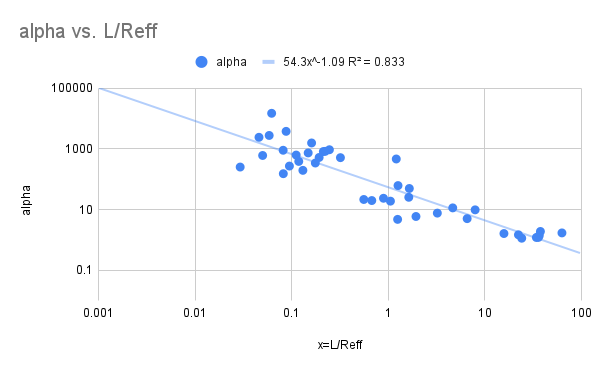
\includegraphics[width=\linewidth]{alphavL_Reff.png} 
\caption{  Free-parameter correlation   }
\label{alpha2}
\end{figure}  
 


We might assume that $\alpha$ is a ratio of the same quantity for  the Milky Way $\rho_{mw}$ with respect to the other   galaxy $\rho_{gal}$  

\begin{equation}
\alpha=\left(\frac{\rho_{mw}}{\rho_{gal}}\right)^{b}  ,
\label{correl}
\end{equation}

as other quantities in this formalism.
 
%\subsection{MOND  \& RAR Comparison}

While reported error    estimates on rotation curve velocities  have not been standardized across the field~\citep{Blok,Gent},     one can reliably   compare fits to the same data with the same  errors. The     reduced $\chi^2_r$ values in table (REF TABLE), demonstrates that the RCFM reduced $\chi^2$ values are twice as low on average as those of the RAR fits  \cite{McGaugh2016RAR}.


 
 \section{  Conclusions \label{sec:conclu}  }
 

This heuristic replacement of dark matter is not a fundamental derivation, but    one supposes if it is possible to quantify these
excesses in shifted spectra using only luminous mass as we do in this paper,  then a       derivation from first principles should   exist.  The curious conspiracy of the luminous mass to   determine the dark matter  is here   compactly explained and characterized as the imprint of our Milky Way on Doppler shifted spectra we receive from external galaxies. Not only is this a more efficient way to predict rotations curves as judged by the average reduced $\chi^2$ in this paper and a smaller free parameter space, but it is also a  more conservative approach than models which require modifications of classical physics  \cite{de_Blok_2010}.  
  
 
 

  
 
%Places where dark matter is invoked. Structure formation: put spherical model replace flat, solve. Galaxy clusters, same,put flow lines on surfaces supported by dark energy. Tully Fisher: temp dependence with mass - but read Beckenstein's description carefully. Hemakes some points.  
   
  The model presented here  is falsifiable if ``dark matter'' effects are   found to be necessary in our Milky Way outside of 8kpc. At the current date, the data of our Milky Way rotation curve is ambiguous outside of our position in the galactic disk.   Recent large surveys of millions of  stars in the Milky Way will differentiate these models   \cite{2022ApJS..259...35A}, \cite{2010ApJ...716....1B}.
  
  
  % We propose   that the other places  where dark matter is invoked     require more complicated  physics assumptions 
      %than are presented here; and can be informed by observations of large scale flows 
     
      %,    and the ``too'' early   formation of galaxies 
     
     % Discrepancies in estimates of the Hubble Flow from supernovae versus from the cosmic microwave background (CITE) and (WHAT"S THE OTHER ISSUE YO). DO I want to include this? 
      
     % MOND      has a fascinating, compact explanation for another dark matter paradox, the  
  % Tully-Fisher relation \cite{1977A&A....54..661T,McGaugh_2000}, but that also is beyond the scope of the current work unfortunately.   
 %In example, the James Webb Space Telescope may have already falsified dark matter driven galaxy formation \cite{2022arXiv221014915H}.
   

%%%%%%
%%%%%
%%%
%%
%
%%%%%%


 % \caption{Results   for SPARC Luminous mass profiles  [NOT UPDATED]\label{sumRESULTS}}
 % \begin{tabular}{@{}llccccccc@{}}
 % \hline
 %  Galaxy     	  &Ref.~&  \multicolumn{3}{c}{\underline{ Other Model Fit Results}}	& & \multicolumn{3}{c}{\underline{LCM Fit Results }}  \\
%\hline
%   	 	& & &  $M/L_{disk}$		& $\chi^2_r$	&&$M/L$&$r_e$&$\chi^2_r$ \\ 
% \hline
%F 563-1	& 2	%& 			
%					&NFW	&--	 		&-- & 	&1.13 	&2.84 	&0.06 \\
%M 31* 	& 12 	%&7.5
%					&ISO	 	 &7.50		&0.36 & 	&5.88	 &4.80 	&0.04  \\
%M 33		& 5	 %&	K 		
%					& NFW 	&0.70		&2.46&  	 &1.98	 &1.46	& 0.17 \\
%NGC 891*	& 11 	% &3.6$\,\umu$m 
		%			&MaxLight &0.9 			&1.10  & 	 &--  	 &	&0.25 \\ 
%NGC 925 	&3	%&3.6$\,\umu$m
 			%		&ISO 	&0.18		 &2.40& 	&0.92	 &4.35	&0.11 \\
%NGC 2403	 & 3	%& 3.6$\,\umu$m
		%			& NFW	&0.41 	 	&4.56& 	&1.12	 	&2.18		& 0.88 \\
%NGC 2841*  &6-3	% & 3.6$\,\umu$m
%					&  James	&0.74 	 	&0.45 & 	&6.25	  &4.84	&0.11 \\
%NGC 2903  &10	 %&B	   		
%					&MOND   	&3.60 	 	&10.71& 	 &2.2	 	&2.81		&0.47\\
% NGC 3198 & 3 	%&3.6$\,\umu$m
%					 &NFW	&0.80	   	&5.40  &   	 &1.80 	 &5.10	&0.64   \\
%NGC 3521  & 8-6	 %&3.6$\,\umu$m 
%					&MOND	&0.71 	 	&0.97 & 	 &2.13  &3.23	&0.22 \\
%NGC 3726	& 10	%&B 			
%					&MOND	&1.00	 	&3.57& 	&1.06	 &2.70	&0.05 \\
%NGC 3953	& 10	%&B 			
%					&MOND	&2.7		 	&1.35& 	&1.79 	&2.60 	&0.35 \\
%NGC 3992	& 10	%&B 			
%					&MOND	&4.93	 	&0.50& 	&2.45 	 &4.77	&0.04 \\
%NGC 4088	& 10	%&B 			
%					&MOND	&1.16		 	&1.70& 	&5.58	 &2.70	&0.27 \\
%NGC 4138	& 10	%&B 			
%					&MOND	&3.5		 	&2.12& 	&3.67	 &1.46	&0.01 \\
%NGC 5055*	 & 3	%&3.6$\,\umu$m 
%					&  NFW	&0.79	 	&17.23&  	&5.87	 &3.29	&0.69 \\
%NGC 5533*	 & 10 %&B 			
%					&MOND	&0.6		  	&1.57 & 	&7.11 	  &3.23	&0.22  \\
%NGC 5907*	& 10	%&B 			
				%	&MOND	&1.6 		 	 &0.44& 	&2.04	 &3.45	%&0.09 \\
%NGC 6946*	&  10	 %& B			
%					&  MOND	& 0.5		 	&   3.03& 	&1.44 	 &0.76	&0.07  \\ 
%NGC 6946*	&  3	 %& B			
%					&  NFW	& 0.5		 	&   3.03& 	&1.44 	 &0.76	&0.07  \\ 
%NGC 7331	&8	% & 3.6$\,\umu$m
%					&James	&0.4 		 	& 0.45& 	&1.34	 &2.44	&0.09 \\
%NGC 7793  &14	%&B			
%					&ISO		&2.6		 	&1.08& 	&2.7	 &1.51	&0.11 \\
%NGC 7814* &11 	% & 3.6$\,\umu$m
%					&ISO   	& 0.68  	 	& 0.25& 	 &-- 	   &	&0.20 \\ 
%UGC 128		&6	%&				
	%				&James	&			&	&	&1.58	  &10.3	%&0.20\\
%UGC 6973	& 10	%&B 			
%					&MOND	&2.7		 	&23.5 & 	&--  	& 	&0.06 \\
%UGC 7524	& 6	%&B 			
%					&James	&--		 	&-- & 	&2.10 	&3.32 	&0.06 \\
% 1.~\citet{Bege}, 2.~\citet{JNav}, 3.~\citet{Blok} , 4.~\citet{Maria}, 
%5.~\citet{Cor03}, 6.~\citet{James},   7.~\citet{Batt},   8.~\citet{Gent},   9.~\citet{Bot},   10.~\citet{SanMcGa},
 % 11.~\citet{Frat},   12.~\citet{Car},   13.~\citet{giraud2000universal},   14.~\citet{Dicaire}, %15.~\cite{Klypin}. \\
%    \end{minipage}
%\end{table*} 


   

  \section[]{Acknowledgments}
 This work is dedicated to Emmett Till, with respect and gratitude to the first nations 
 on whose lands this was written; 
  the Coast Salish Peoples of Washington State, 
 the Cheyenne,
 Arapaho and Ute  Peoples of Colorado, and the Algonquian Peoples of Massachusetts.  

  The authors would like to thank  S.\ McGaugh,  V.\,P.\,  Nair,   R.\, Walterbos,  A.\, Klypin, K. Bender, C. Beetle and     T.\, Boyer.   \\
  
 
% QUESTION FOR GROUP: how is our model predictive, more so than MOND, since we both do well on fitting galaxies. The Milky Way. We get a large enough sample of galaxies with certain distances and good photometry (SPARC) and run against a two MW. 

%%%%%%%
\clearpage

\begin{figure}
\centering
\begin{minipage}{.5\textwidth}
  \centering
  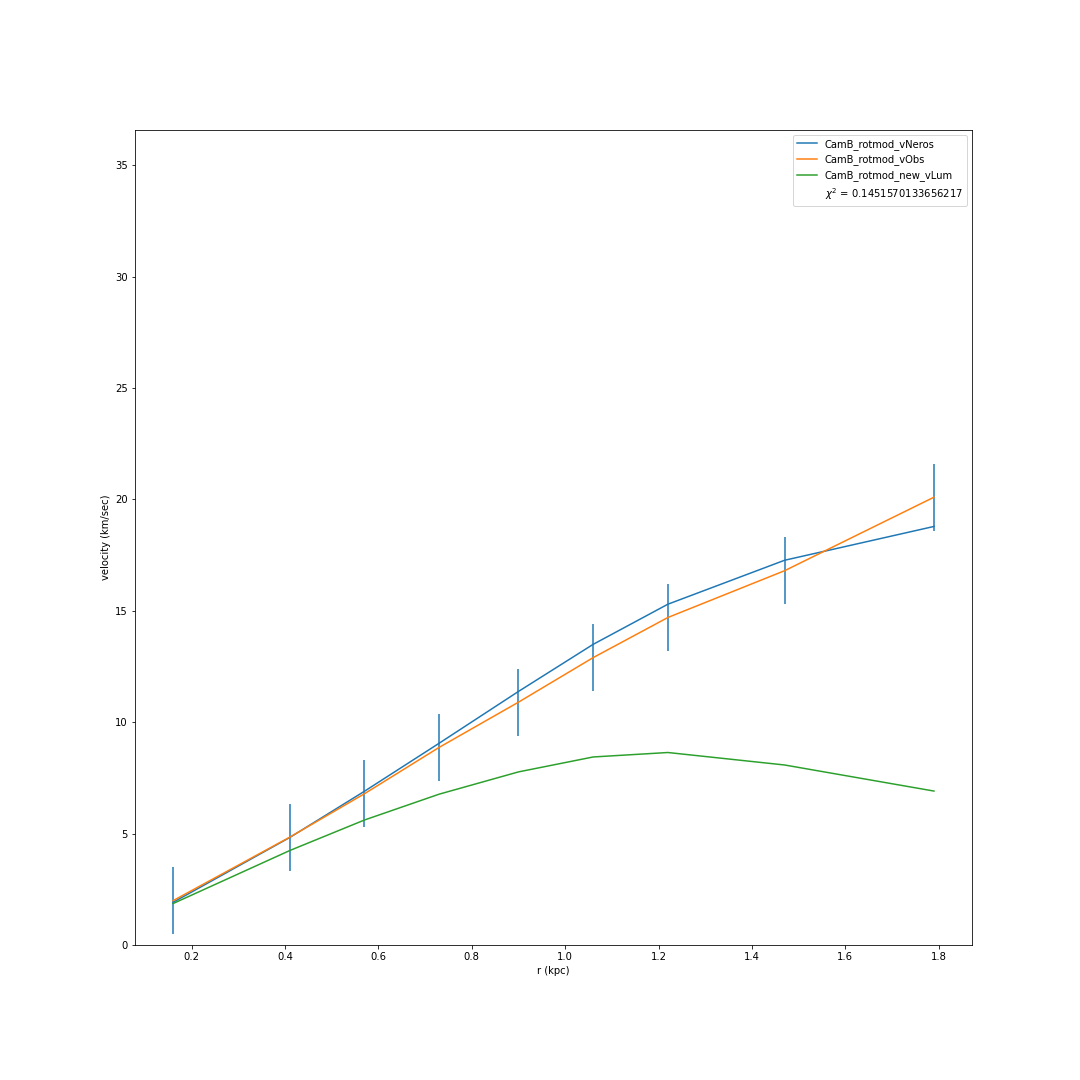
\includegraphics[width=.49\linewidth]{figures/CamB_rotmod_XueSofue.png}
  \captionof{figure}{CamB : SPARC\cite{2016Lelli}}
  \label{fig:test1}
\end{minipage}%
\begin{minipage}{.5\textwidth}
  \centering
  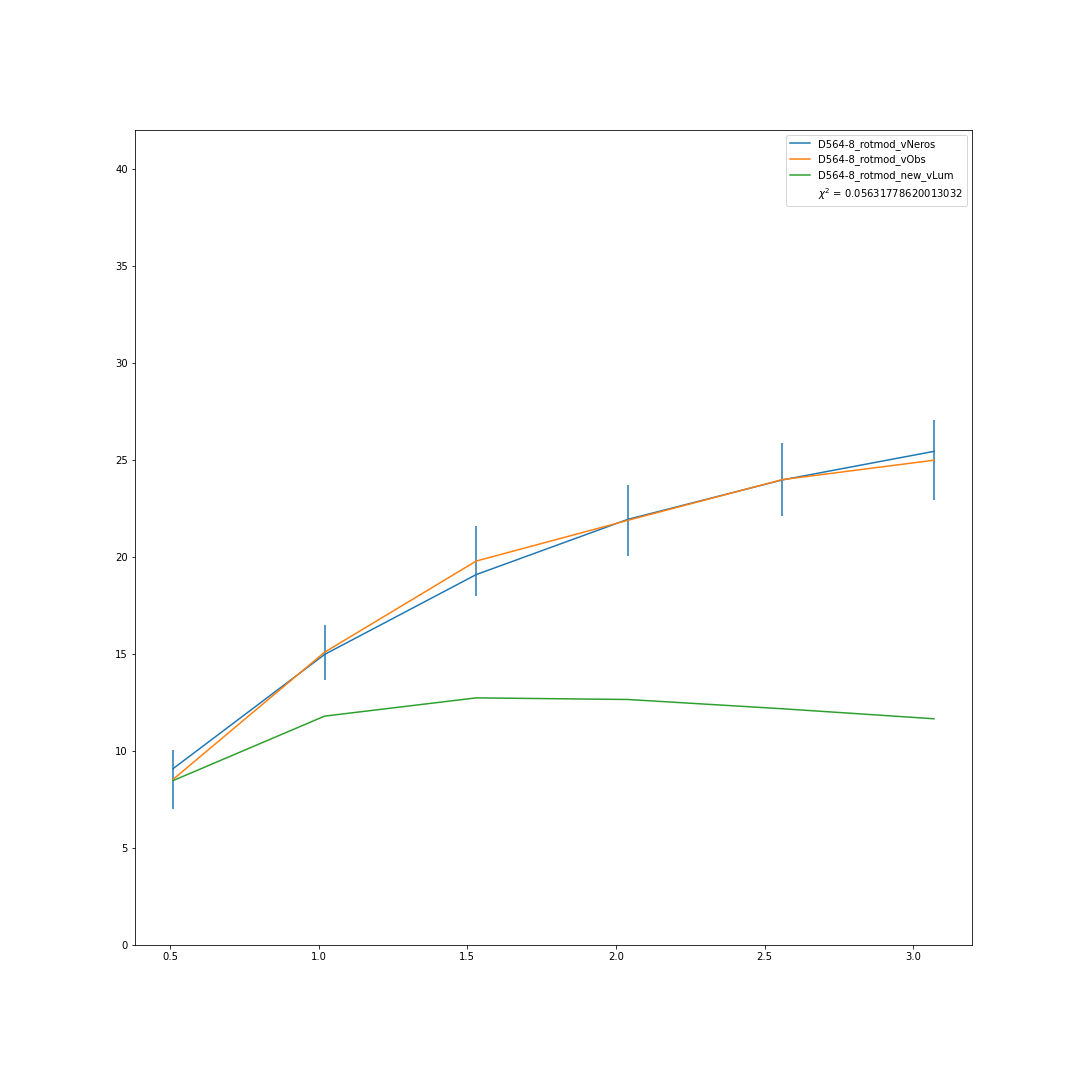
\includegraphics[width=.49\linewidth]{figures/D564-8_rotmod_XueSofue.png}
  \captionof{figure}{D564-8 : SPARC\cite{2016Lelli}e}
  \label{fig:test2}
\end{minipage}
\begin{minipage}{.5\textwidth}
  \centering
  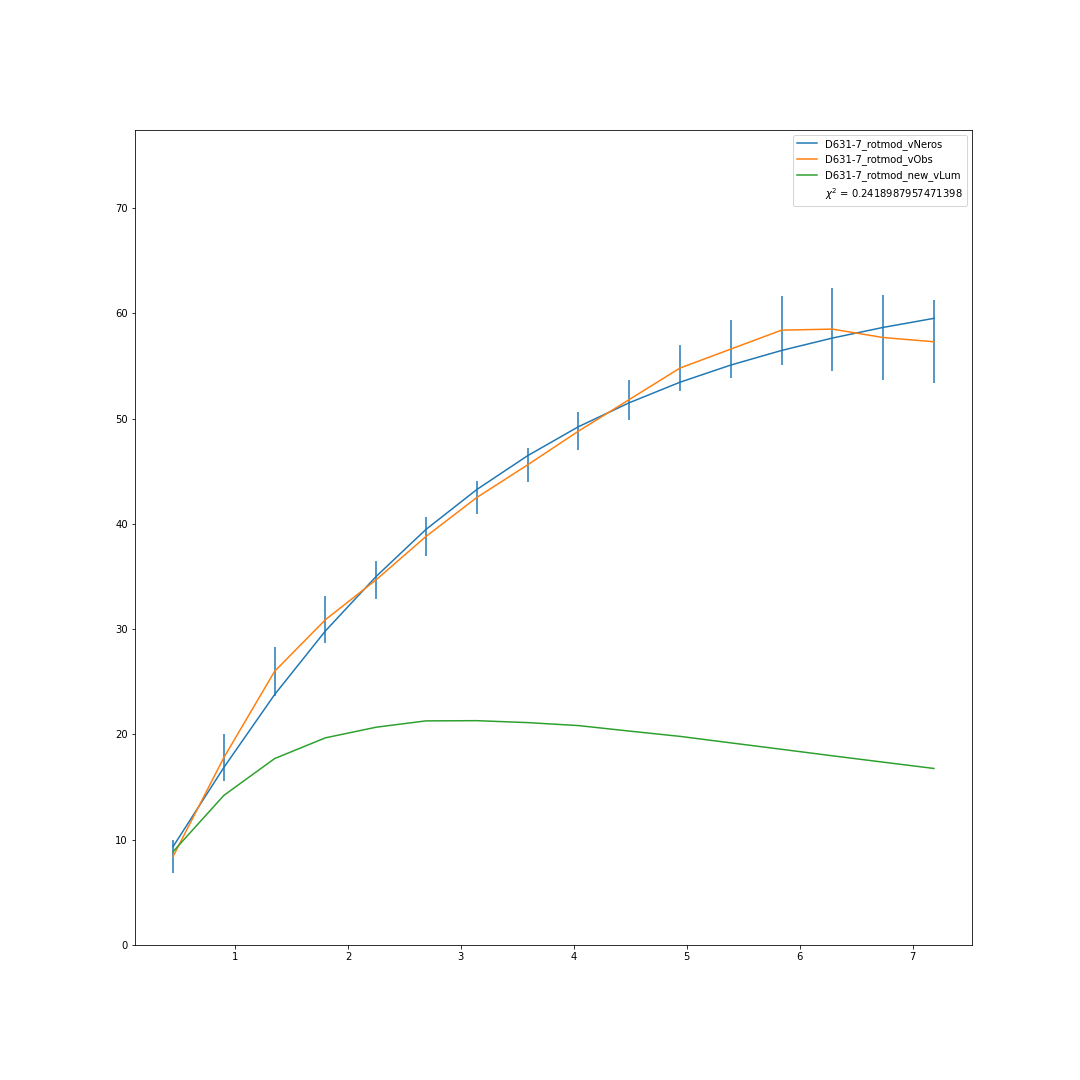
\includegraphics[width=.4\linewidth]{figures/D631-7_rotmod_XueSofue.png}
  \captionof{figure}{D631-7  SPARC\cite{2016Lelli}}
  \label{fig:test1}
\end{minipage}%
\begin{minipage}{.5\textwidth}
  \centering
  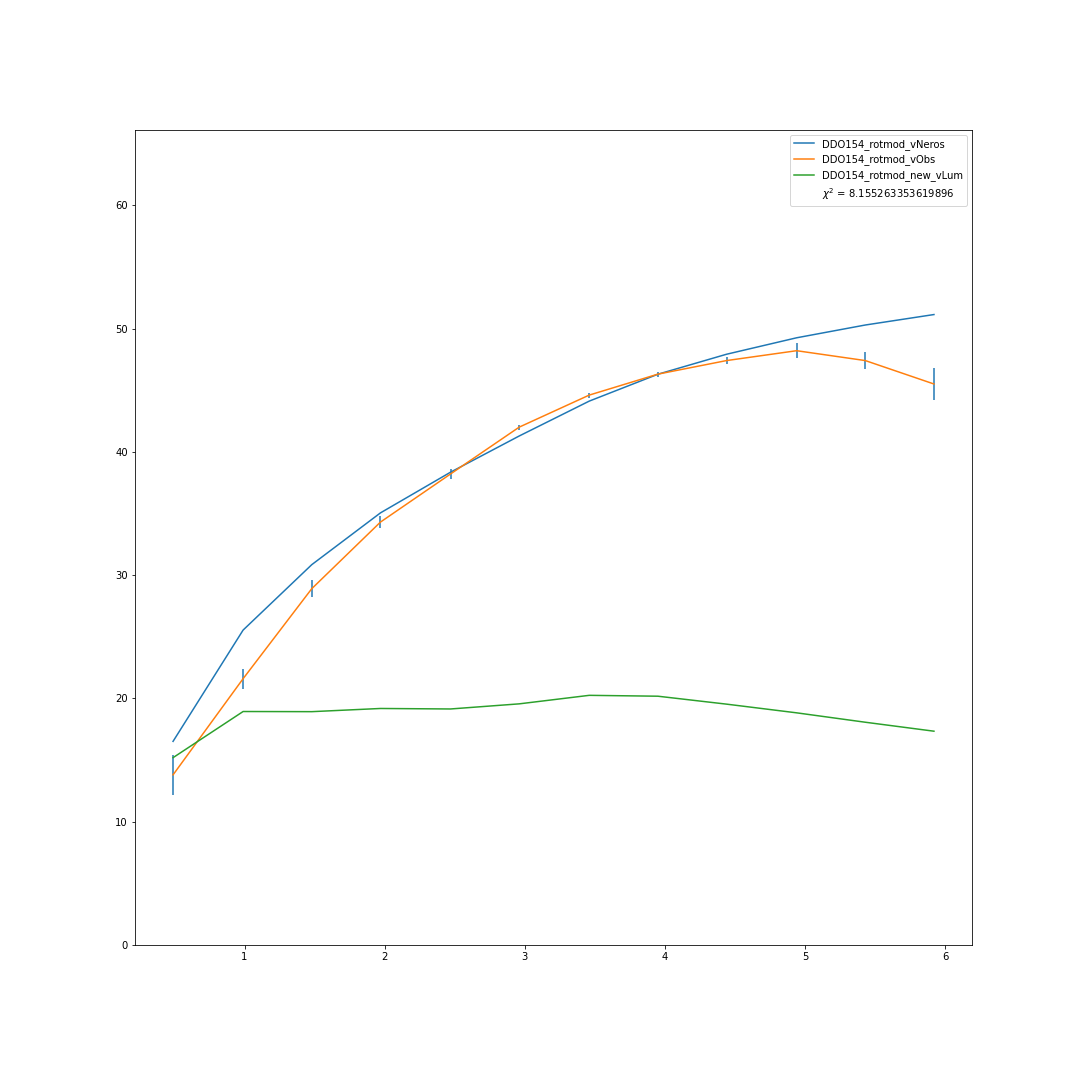
\includegraphics[width=.4\linewidth]{figures/DDO154_rotmod_XueSofue.png}
  \captionof{figure}{DD00154 : SPARC\cite{2016Lelli}e}
  \label{fig:test2}
\end{minipage}
\begin{minipage}{.5\textwidth}
  \centering
  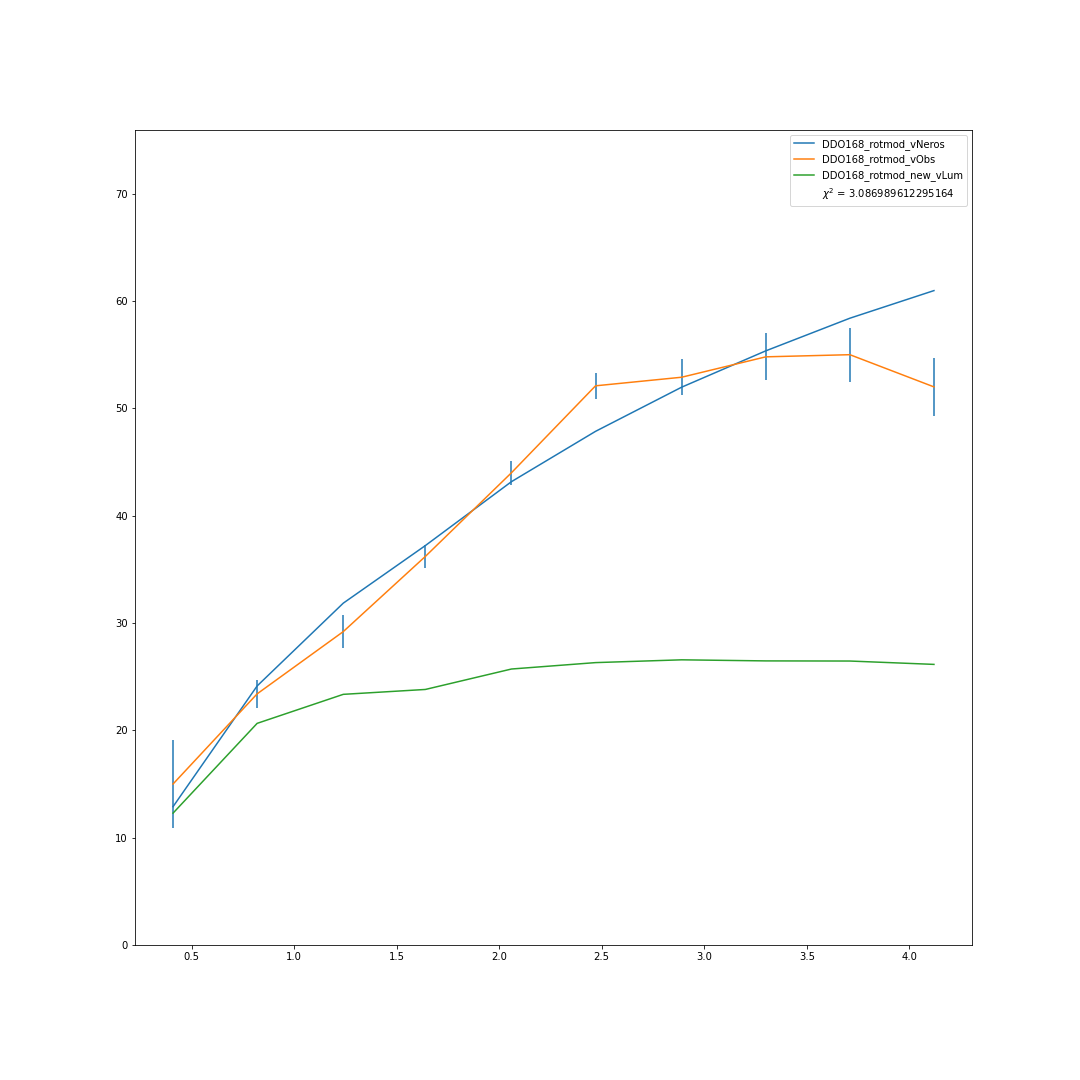
\includegraphics[width=.8\linewidth]{figures/DDO168_rotmod_XueSofue.png}
  \captionof{figure}{DDO168  SPARC\cite{2016Lelli}}
  \label{fig:test1}
\end{minipage}%
\begin{minipage}{.5\textwidth}
  \centering
  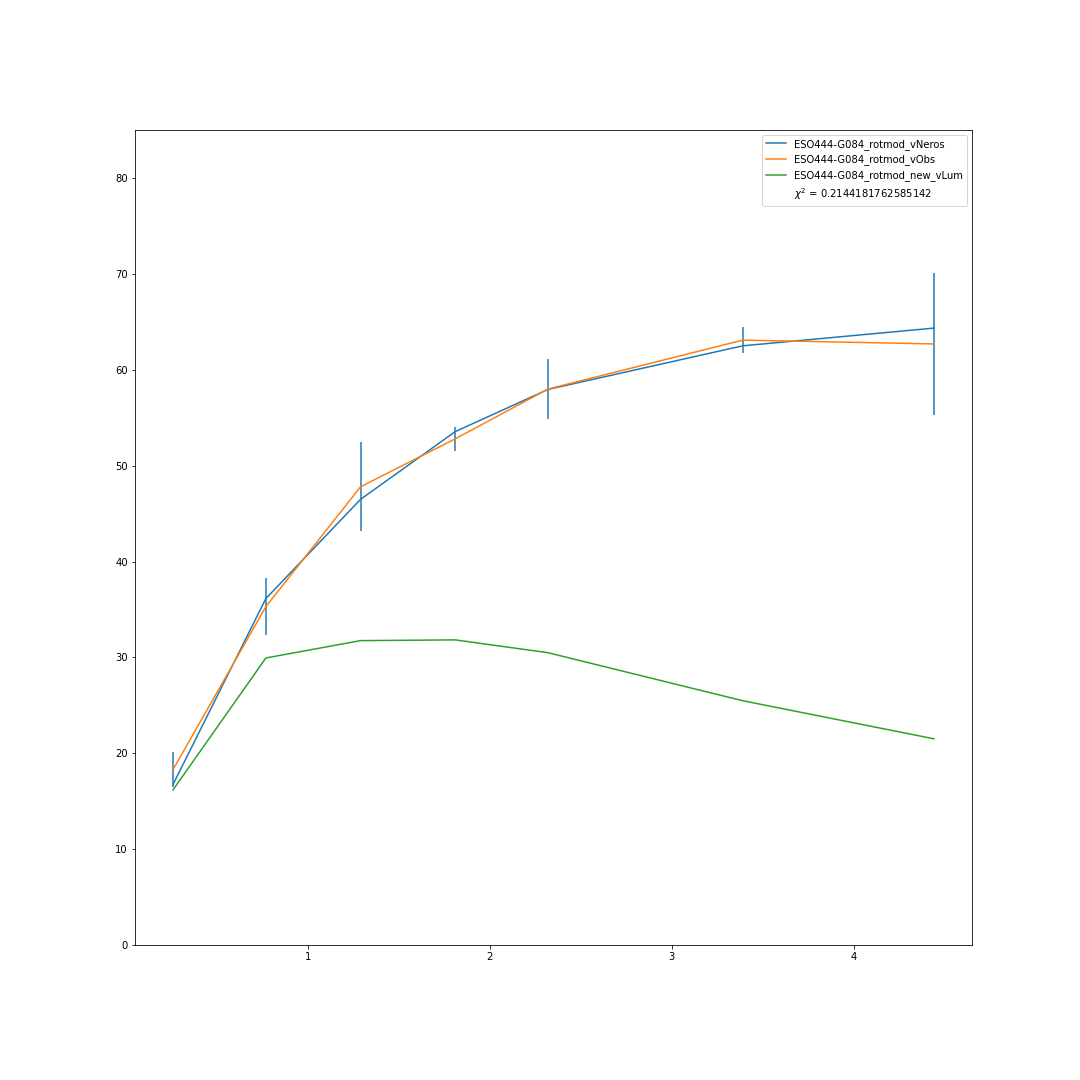
\includegraphics[width=.8\linewidth]{figures/ESO444-G084_rotmod_XueSofue.png}
  \captionof{figure}{ESO444-G084 : SPARC\cite{2016Lelli}}
  \label{fig:test2}
\end{minipage}
\end{figure}

 
  %%%%%%%
\begin{figure} 
\centering
\begin{minipage}{0.5\textwidth}
%\centering
  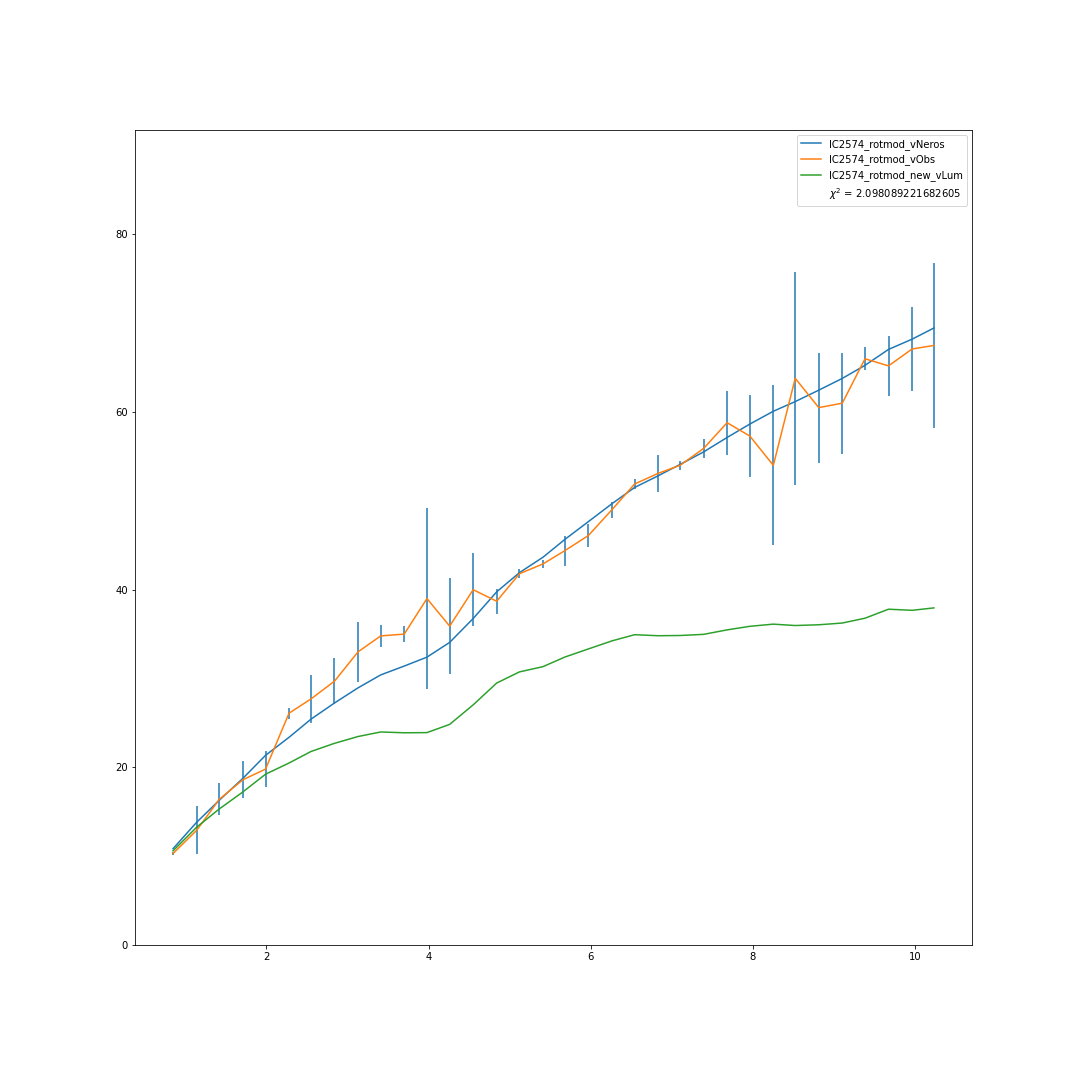
\includegraphics[width=.8\linewidth]{figures/IC2574_rotmod_XueSofue.png}
\caption{ SPARC\cite{2016Lelli}}
\label{fig:2841}
\end{minipage}
\begin{minipage}{0.5\textwidth}
%\centering
  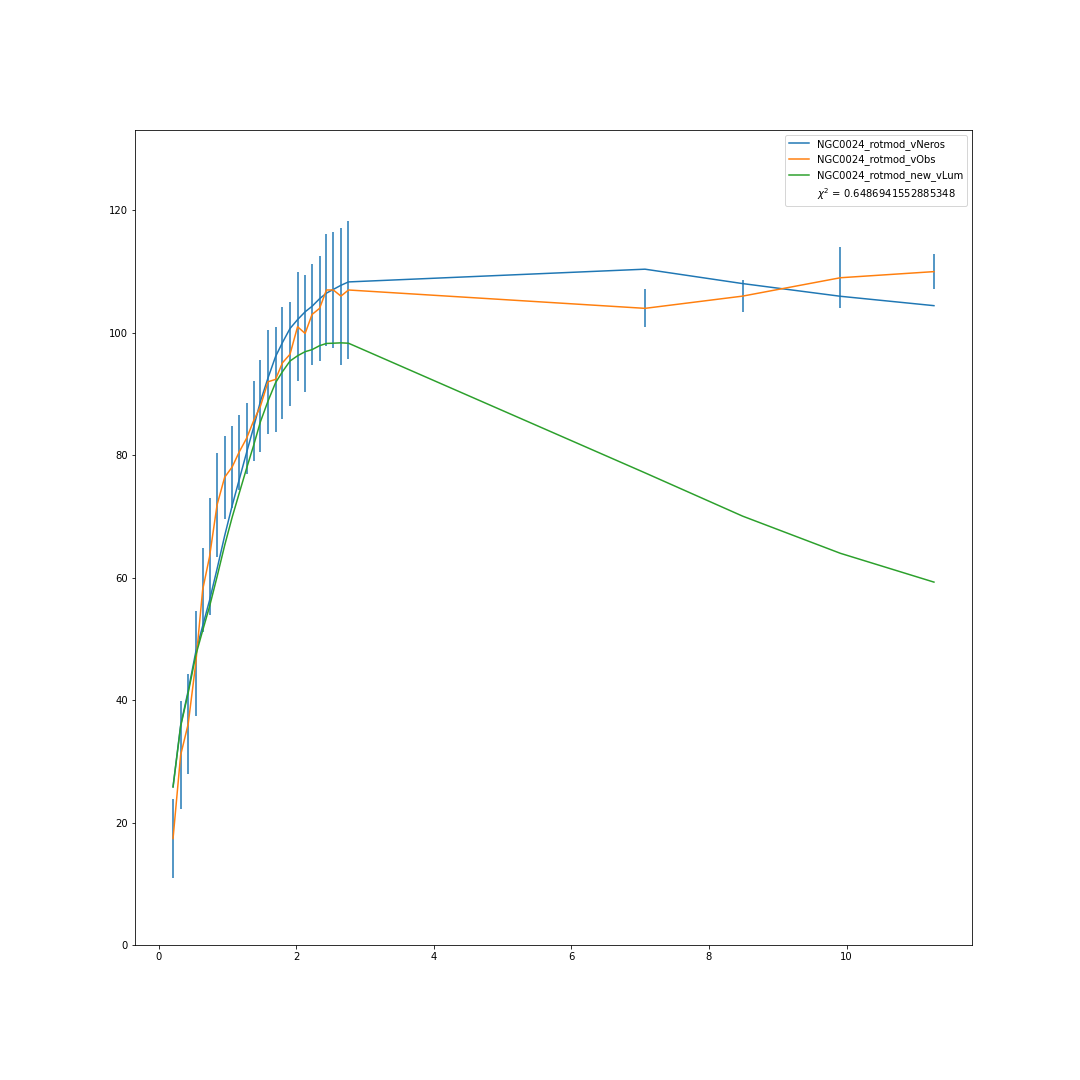
\includegraphics[width=.8\linewidth]{figures/NGC0024_rotmod_XueSofue.png}
\caption{ SPARC\cite{2016Lelli}}
\label{fig:2915}
\end{minipage}
\end{figure}
%%%%%%%
\begin{figure} 
\centering
\begin{minipage}{0.5\textwidth}
%\centering
  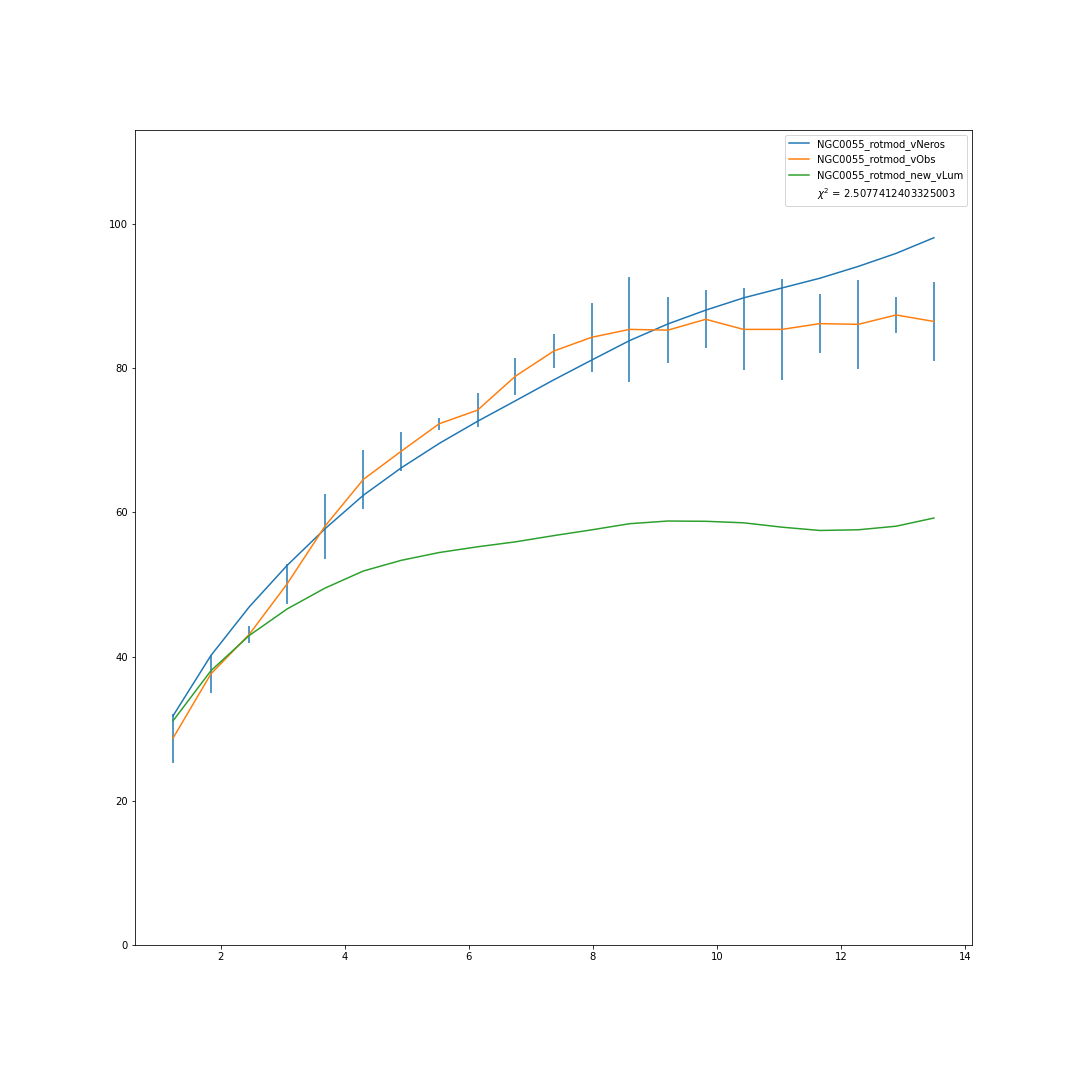
\includegraphics[width=.8\linewidth]{figures/NGC0055_rotmod_XueSofue.png}
\caption{ SPARC\cite{2016Lelli}}
\label{fig:2841}
\end{minipage}
\begin{minipage}{0.5\textwidth}
%\centering
  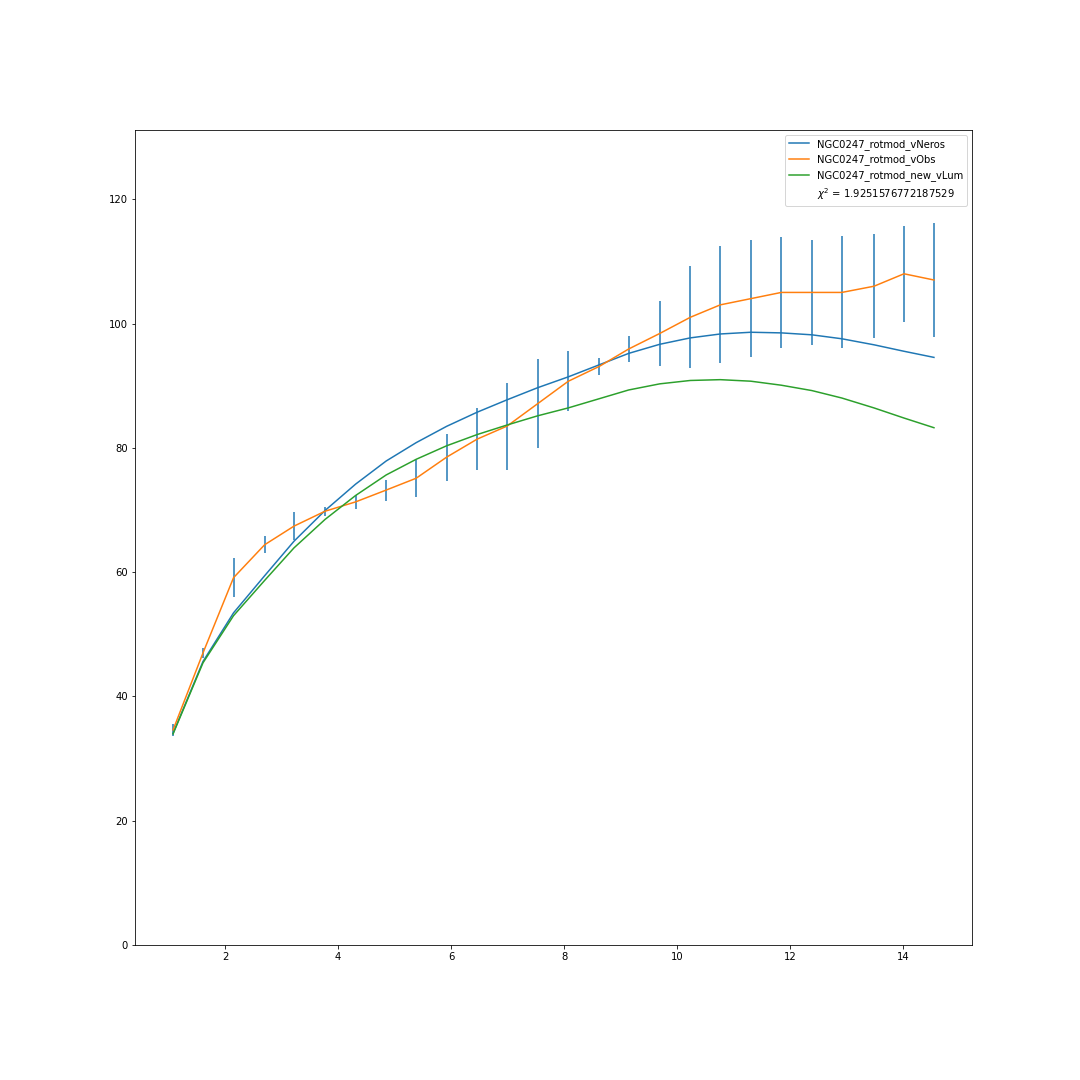
\includegraphics[width=.8\linewidth]{figures/NGC0247_rotmod_XueSofue.png}
\caption{ SPARC\cite{2016Lelli}}
\label{fig:2915}
\end{minipage}
\end{figure}
%%%%%%%
 %%%%%%%
\begin{figure} 
\centering
\begin{minipage}{0.5\textwidth}
%\centering
  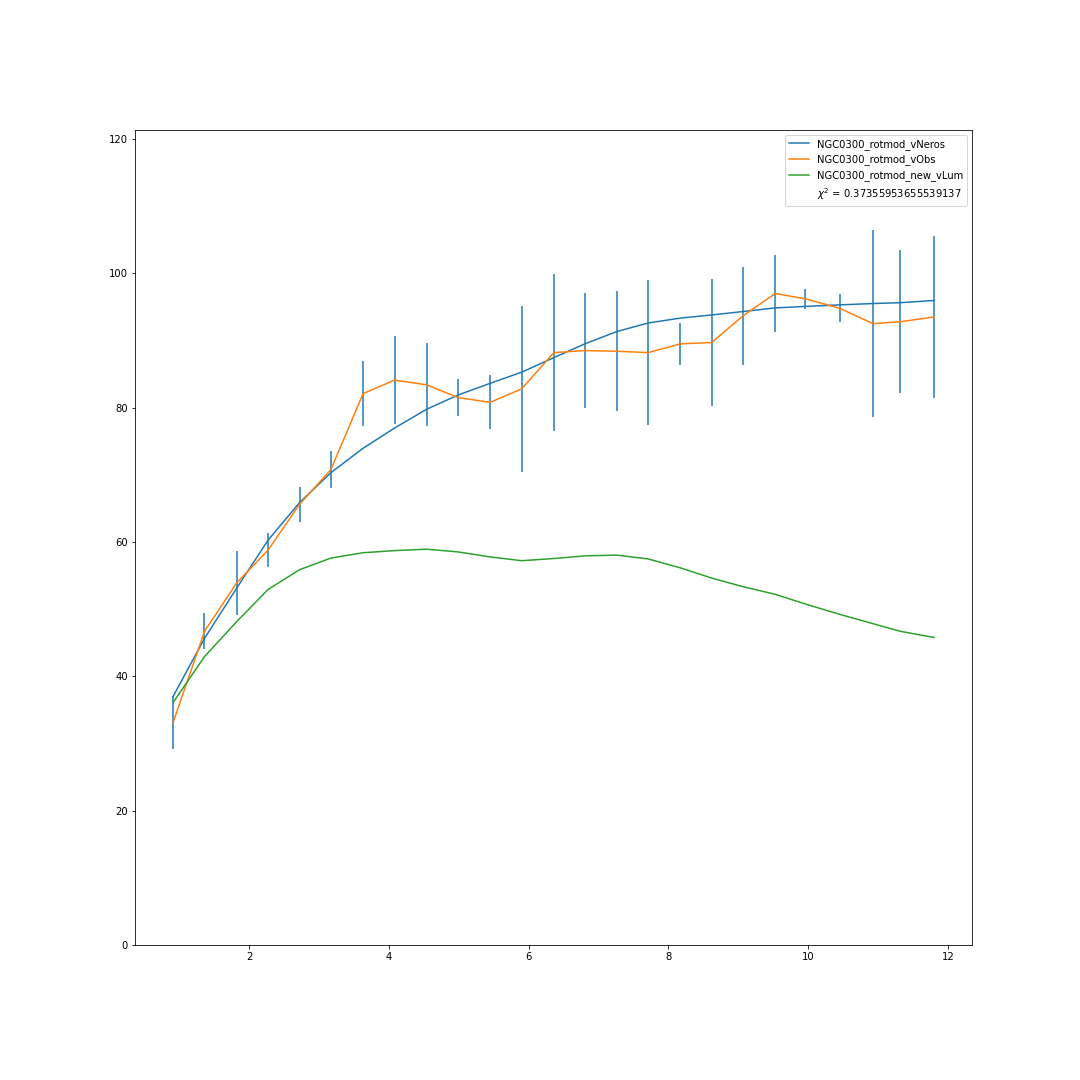
\includegraphics[width=.8\linewidth]{figures/NGC0300_rotmod_XueSofue.png}
\caption{ SPARC\cite{2016Lelli}}
\label{fig:2841}
\end{minipage}
\begin{minipage}{0.5\textwidth}
%\centering
  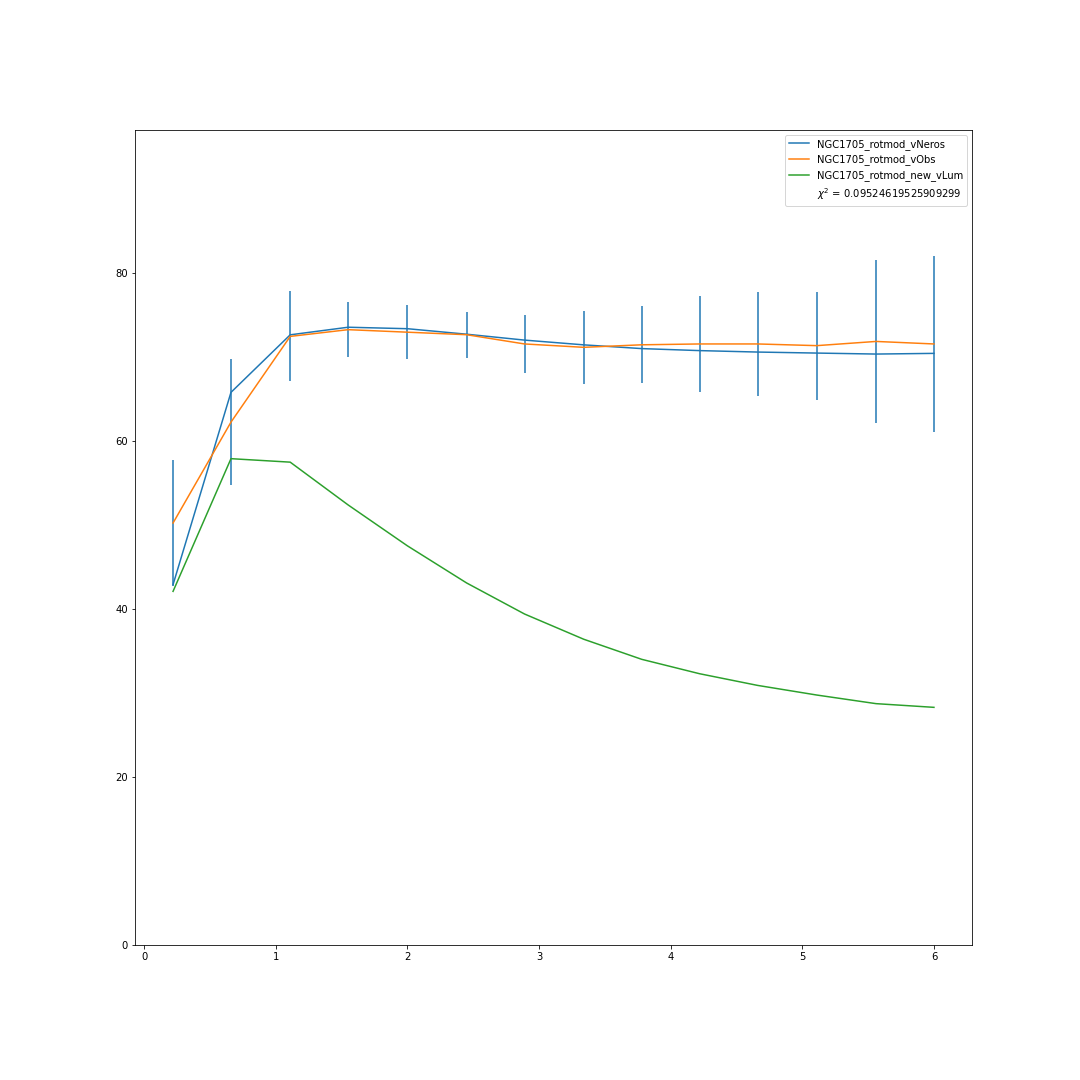
\includegraphics[width=.8\linewidth]{figures/NGC1705_rotmod_XueSofue.png}
\caption{ SPARC\cite{2016Lelli}}
\label{fig:2915}
\end{minipage}
\end{figure}
%%%%%%%
 %%%%%%%
\begin{figure} 
\centering
\begin{minipage}{0.5\textwidth}
%\centering
  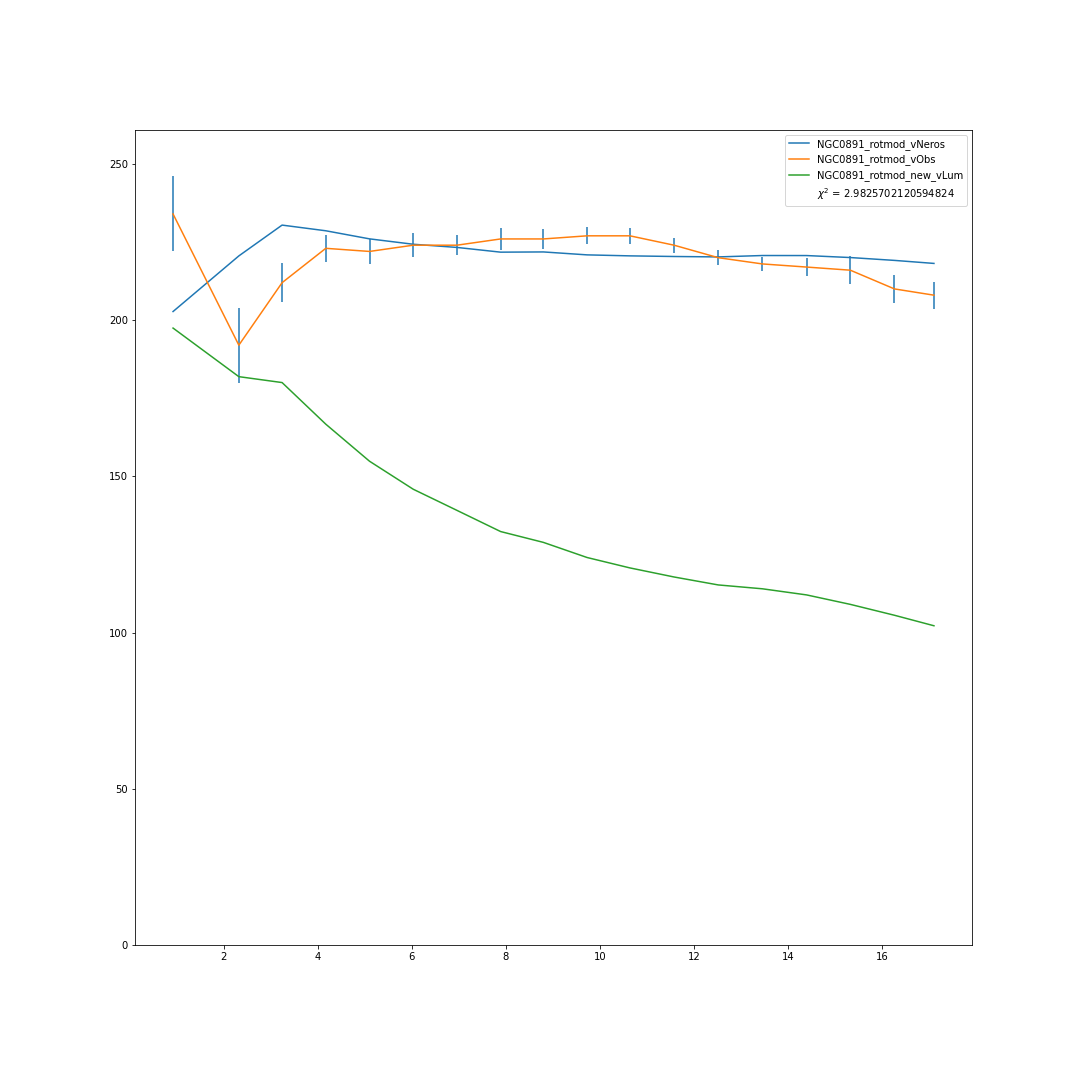
\includegraphics[width=.8\linewidth]{figures/NGC0891_rotmod_XueSofue.png}
\caption{ SPARC\cite{2016Lelli}}
\label{fig:2841}
\end{minipage}
\begin{minipage}{0.5\textwidth}
%\centering
  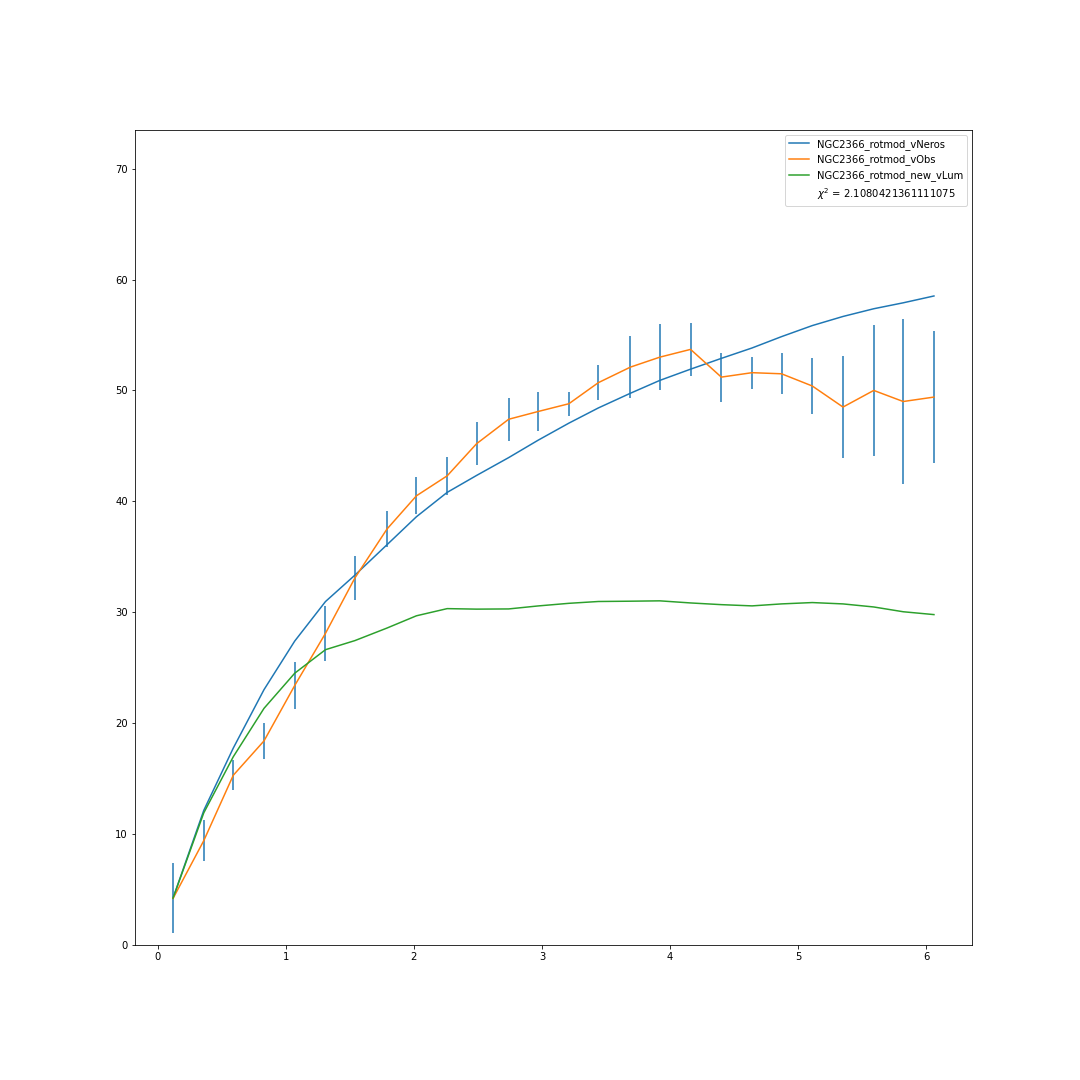
\includegraphics[width=.8\linewidth]{figures/NGC2366_rotmod_XueSofue.png}
\caption{ SPARC\cite{2016Lelli}}
\label{fig:2915}
\end{minipage}
\end{figure}
%%%%%%%

  
   %%%%%%%
\begin{figure} 
\centering
\begin{minipage}{0.5\textwidth}
%\centering
  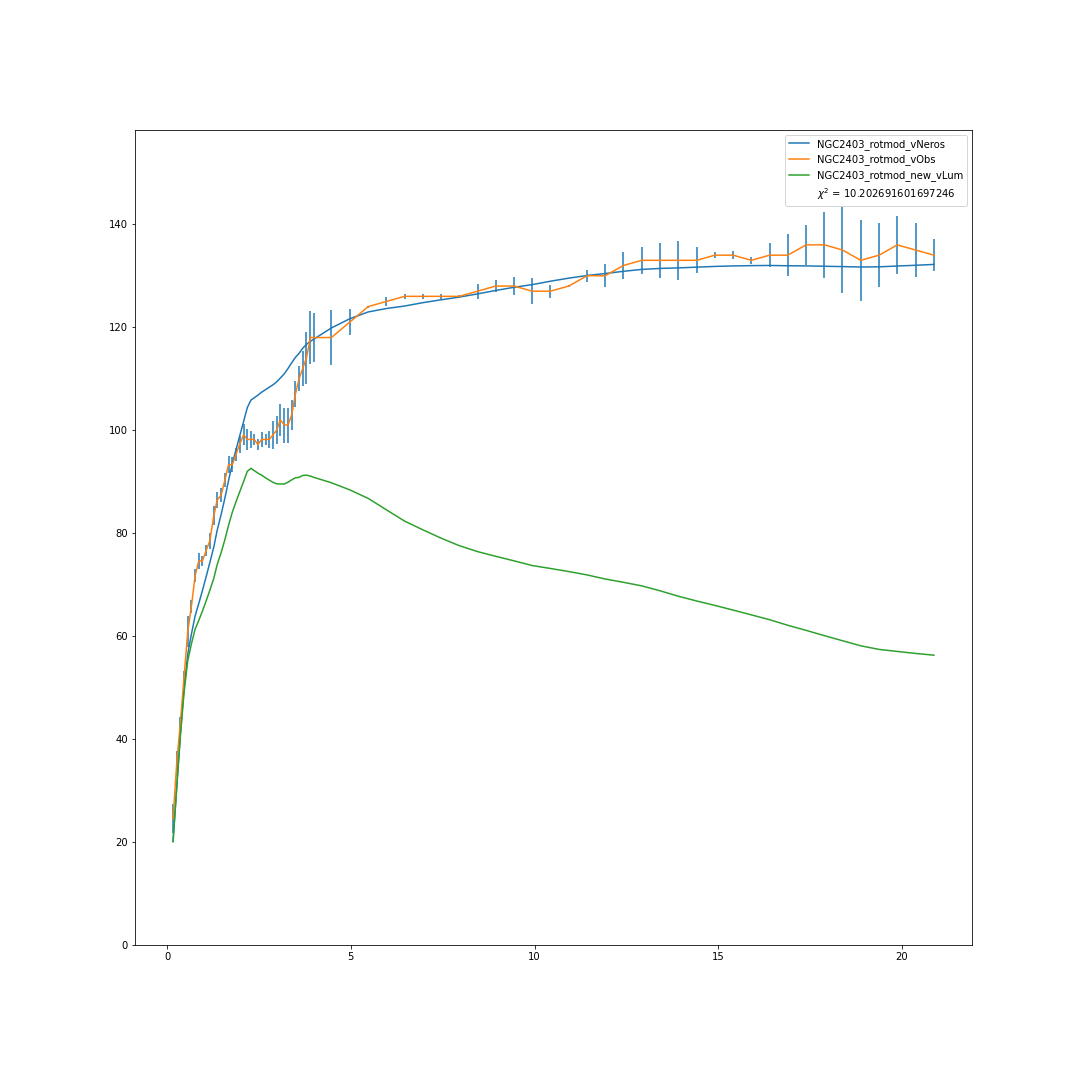
\includegraphics[width=.8\linewidth]{figures/NGC2403_rotmod_XueSofue.png}
\caption{ SPARC\cite{2016Lelli}}
\label{fig:2841}
\end{minipage}
\begin{minipage}{0.5\textwidth}
%\centering
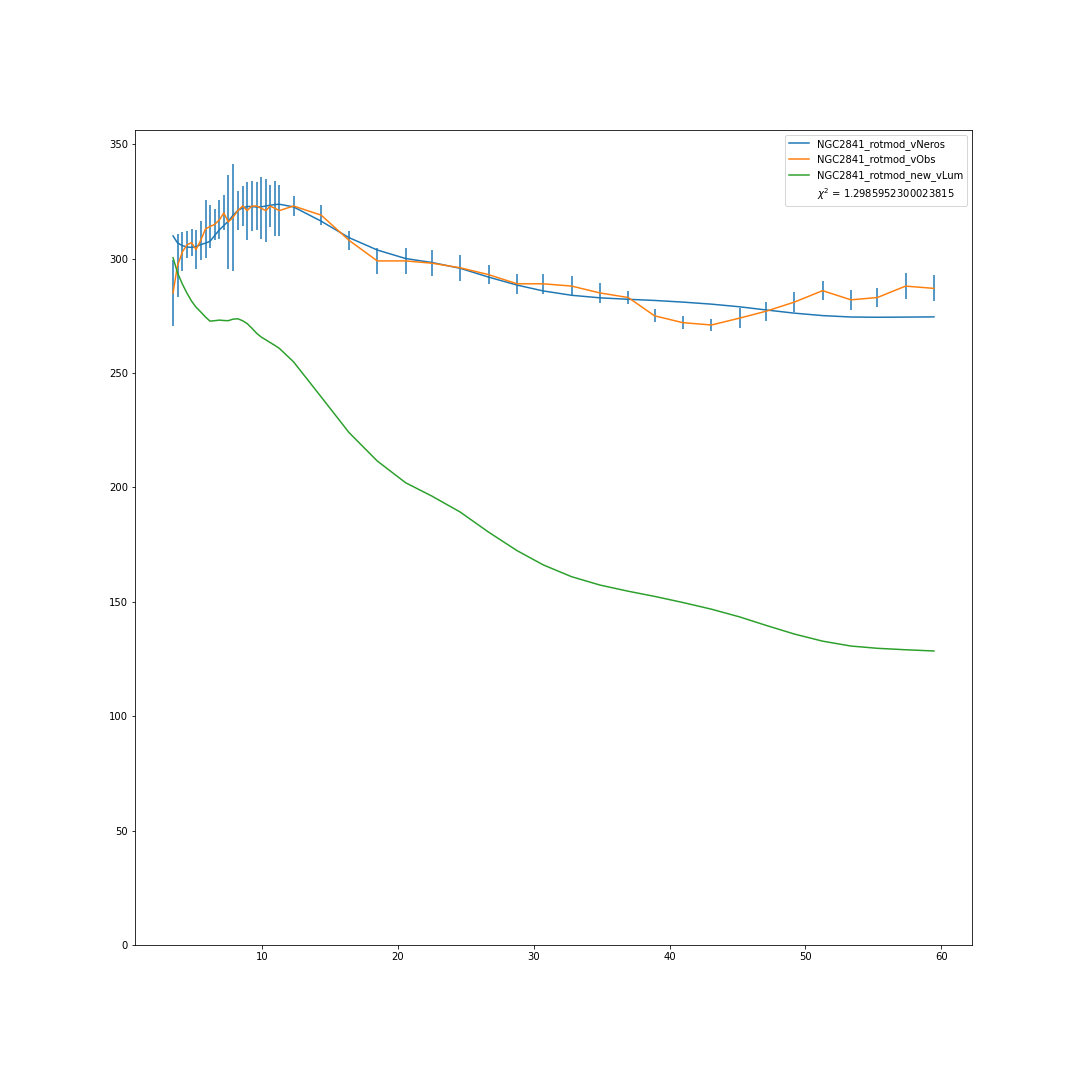
\includegraphics[width=0.43\linewidth]{figures/NGC2841_rotmod_XueSofue.png}
\caption{ SPARC\cite{2016Lelli}}
\label{fig:2915}
\end{minipage}
\end{figure}
%%%%%%%
 
 
%%%%%%%
\begin{figure} 
\centering
\begin{minipage}{0.5\textwidth}
%\centering
\caption{NGC 2841 SPARC\cite{2016Lelli}}
\label{fig:2841}
\end{minipage}
\begin{minipage}{0.5\textwidth}
%\centering
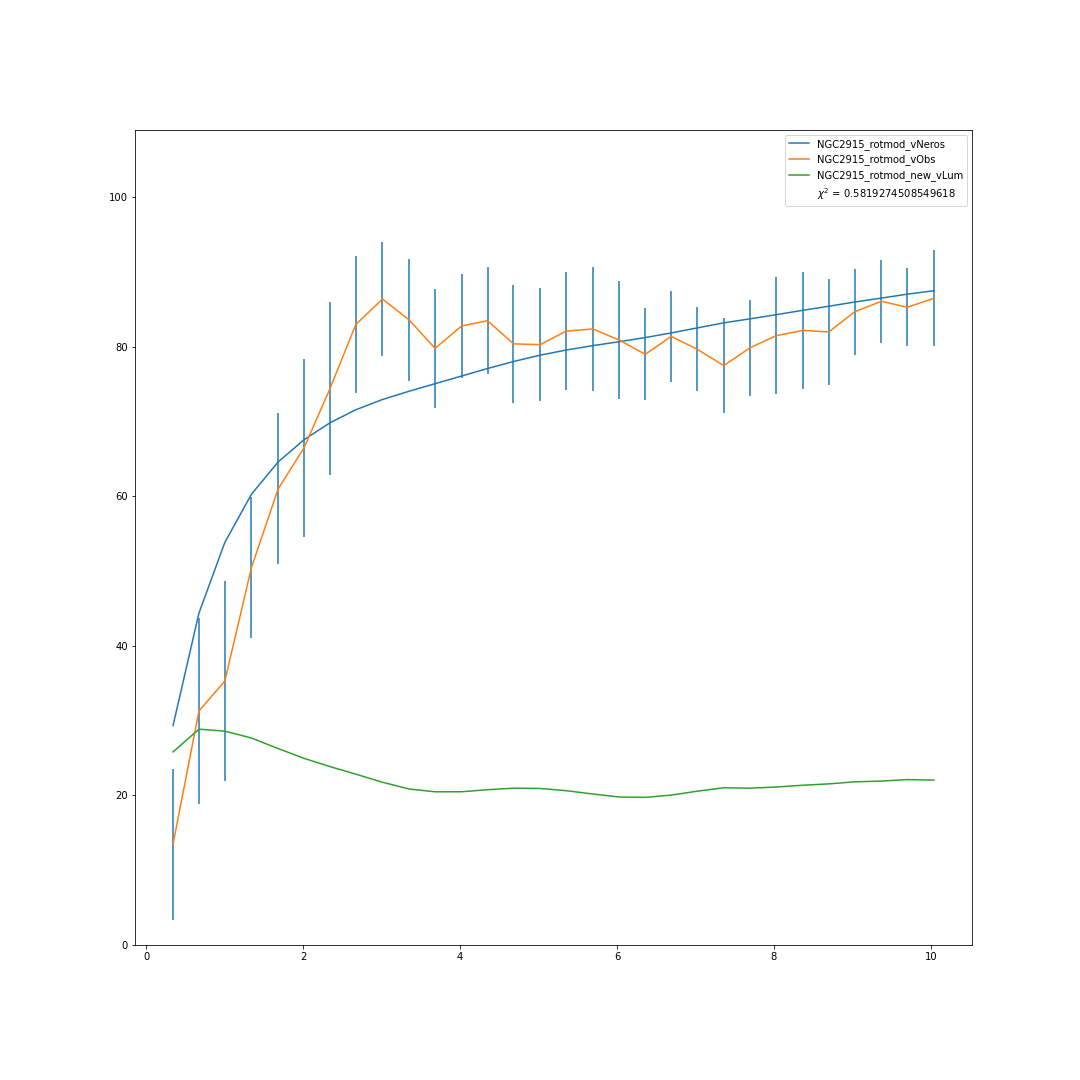
\includegraphics[width=0.43\linewidth]{figures/NGC2915_rotmod_XueSofue.png}
\caption{NGC 2915 SPARC\cite{2016Lelli}}
\label{fig:2915}
\end{minipage}
\end{figure}
%%%%%%%
%
%  
%%%%%%%
\begin{figure} 
\centering
\begin{minipage}{0.5\textwidth}
%\centering
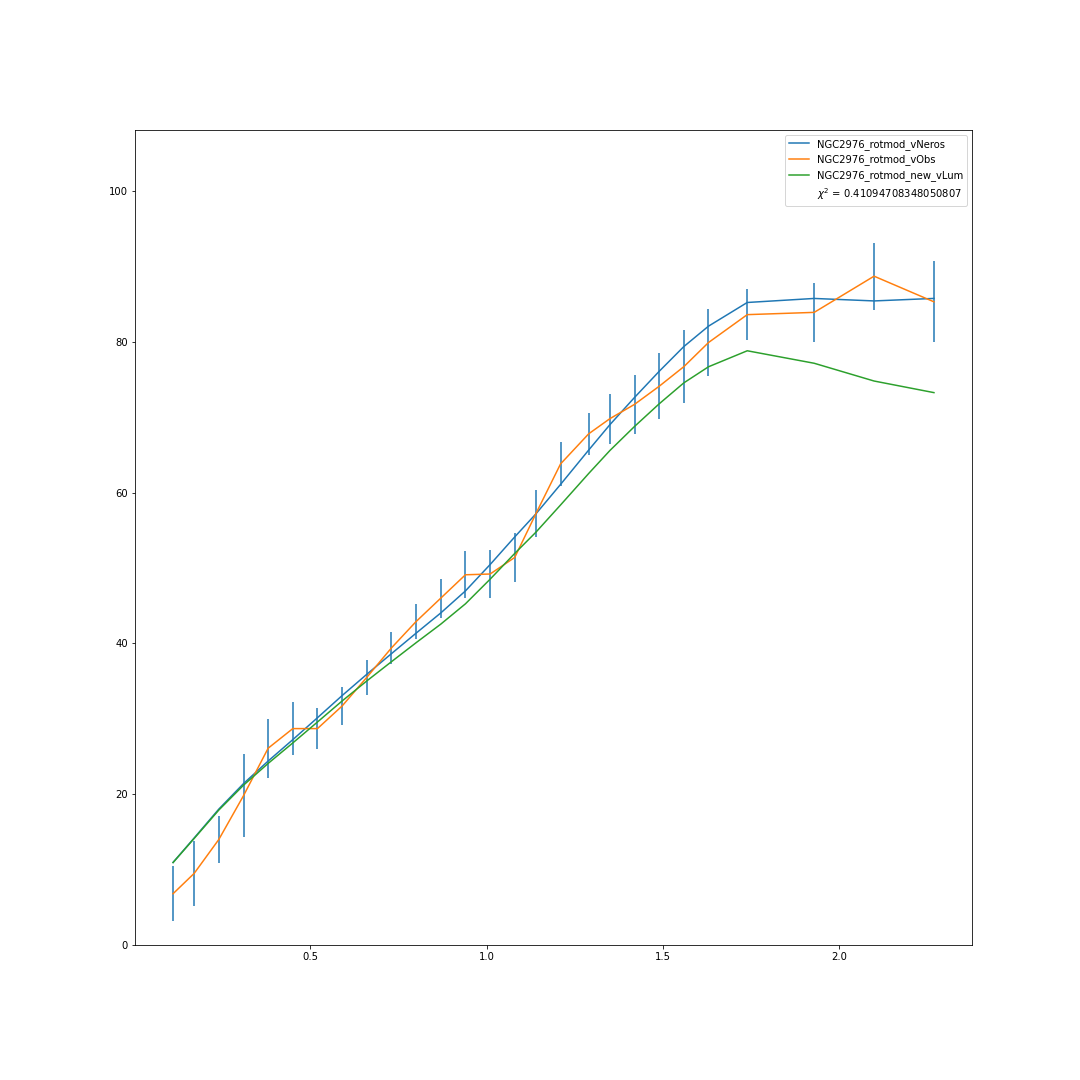
\includegraphics[width=0.43\linewidth]{figures/NGC2976_rotmod_XueSofue.png}
\caption{NGC 2976}
\label{fig:2976}
\end{minipage}
\begin{minipage}{0.5\textwidth}
%\centering
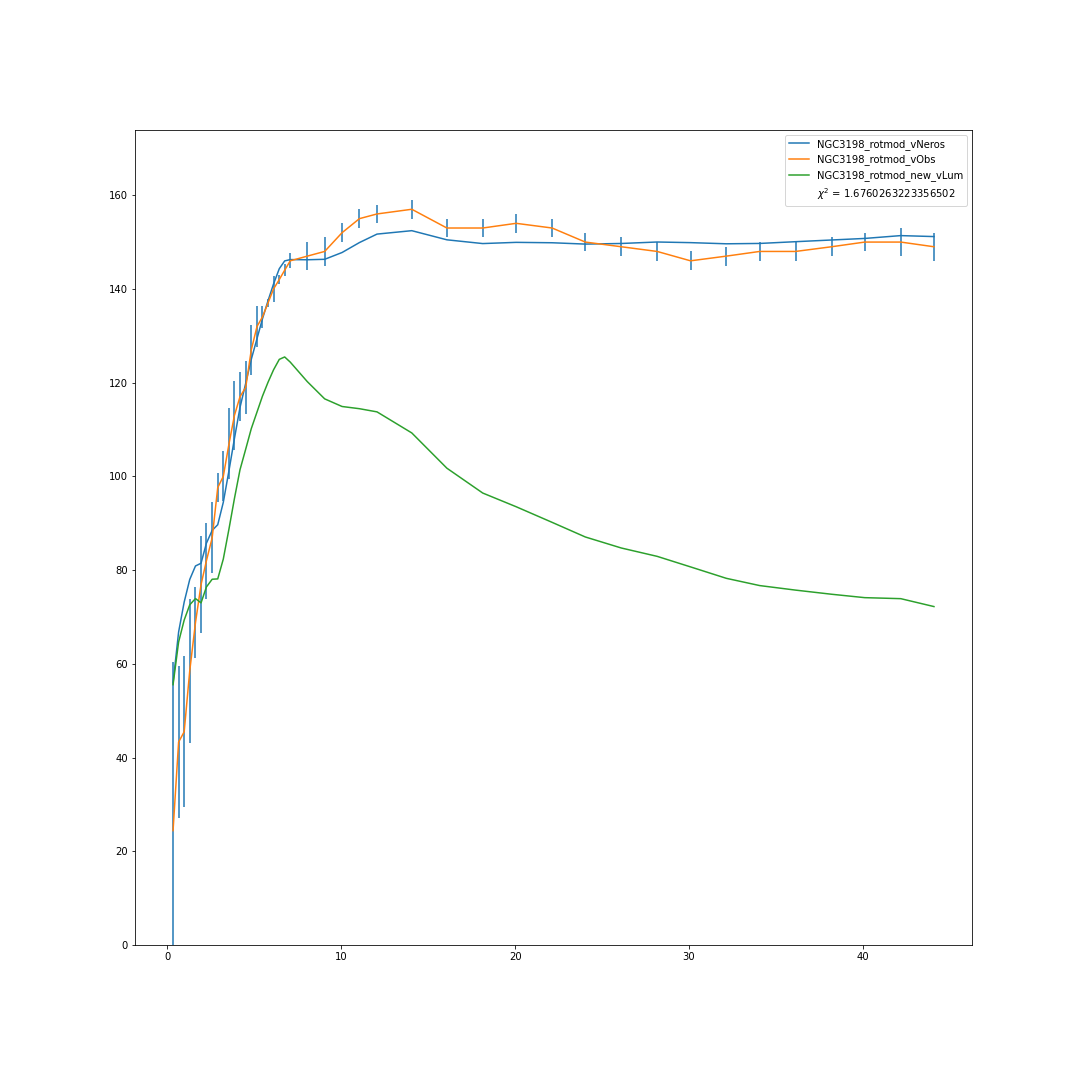
\includegraphics[width=0.43\linewidth]{figures/NGC3198_rotmod_XueSofue.png}
\caption{NGC 3198}
\label{fig:3198}
\end{minipage}
\end{figure}
%%%%%%%
%%%%%%%%
%%%%%%
%%%%%%%
%%%%%%
  
 

    
     

\bibliography{LCM} 

\end{document}
%
% ****** End of file apssamp.tex ******